\section{Construção de uma heap binária em $O(N)$ }

\begin{frame}[fragile]{Heapify}

    \begin{itemize}
        \item Dado um vetor de elementos \code{c}{xs}, uma \textit{heap} binária pode ser
            construída em $O(N\log N)$ através de $N$ inserções

        \item Porém é possível construir a mesma \textit{heap} em $O(N)$

        \item Esta rotina, denominada \textit{heapify}, foi proposta por Floyd

        \item Ela consiste em preencher uma árvore binária com os elementos de \code{c}{xs},
            na ordem em que foram informados

        \item Em seguida, em ordem reversa (da última folha para a raiz), as violações da
            propriedade fundamental devem ser corrigidas, utilizado a mesma estratégia da
            extração do elemento máximo
    \end{itemize}

\end{frame}

\begin{frame}[fragile]{Exemplo de execução da rotina \code{c}{heapify()}}

    \begin{figure}
        \centering
        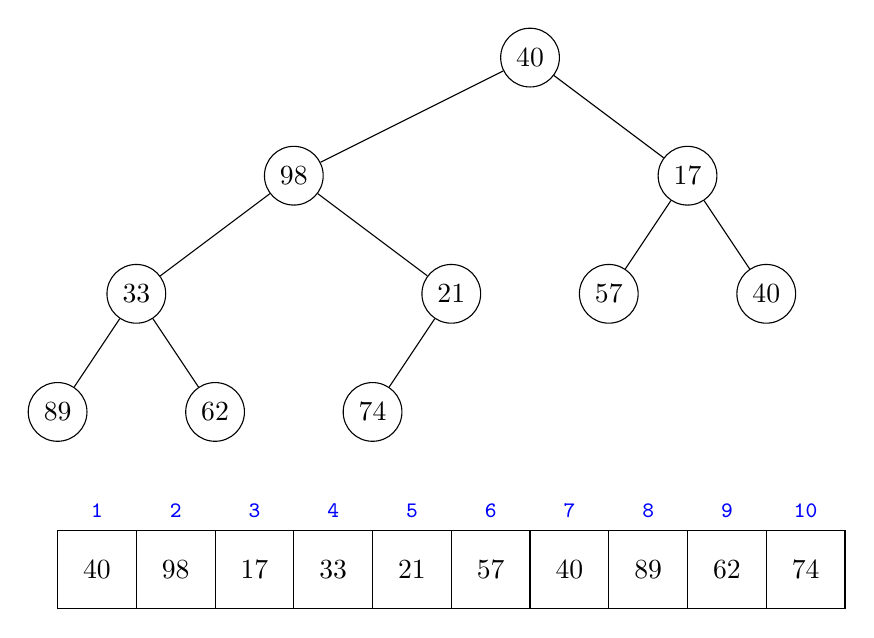
\begin{tikzpicture}
                % Sequência de inserção: 40, 98, 17, 33, 21, 57, 40, 89, 62, 74
                \node[circle,draw] (A) at (6, 6) { 40 };
                \node[circle,draw] (B) at (3, 4.5) { 98 };
                \node[circle,draw] (C) at (8, 4.5) { 17 };
                \node[circle,draw] (D) at (1, 3) { 33 };
                \node[circle,draw] (E) at (5, 3) { 21 };
                \node[circle,draw] (F) at (7, 3) { 57 };
                \node[circle,draw] (G) at (9, 3) { 40 };
                \node[circle,draw] (H) at (0, 1.5) { 89 };
                \node[circle,draw] (I) at (2, 1.5) { 62 };
                \node[circle,draw] (J) at (4, 1.5) { 74 };

                \draw (A) -- (B);
                \draw (A) -- (C);
                \draw (B) -- (D);
                \draw (B) -- (E);
                \draw (C) -- (F);
                \draw (C) -- (G);
                \draw (D) -- (H);
                \draw (D) -- (I);
                \draw (E) -- (J);

                \draw (0, -1) grid (10, 0);

                \node[color=blue] at (0.5, 0.25) { \footnotesize \texttt{\textbf{1}} };
                \node[color=blue] at (1.5, 0.25) { \footnotesize \texttt{\textbf{2}} };
                \node[color=blue] at (2.5, 0.25) { \footnotesize \texttt{\textbf{3}} };
                \node[color=blue] at (3.5, 0.25) { \footnotesize \texttt{\textbf{4}} };
                \node[color=blue] at (4.5, 0.25) { \footnotesize \texttt{\textbf{5}} };
                \node[color=blue] at (5.5, 0.25) { \footnotesize \texttt{\textbf{6}} };
                \node[color=blue] at (6.5, 0.25) { \footnotesize \texttt{\textbf{7}} };
                \node[color=blue] at (7.5, 0.25) { \footnotesize \texttt{\textbf{8}} };
                \node[color=blue] at (8.5, 0.25) { \footnotesize \texttt{\textbf{9}} };
                \node[color=blue] at (9.5, 0.25) { \footnotesize \texttt{\textbf{10}} };

                \node at (0.5, -0.5) { 40 };
                \node at (1.5, -0.5) { 98 };
                \node at (2.5, -0.5) { 17 };
                \node at (3.5, -0.5) { 33 };
                \node at (4.5, -0.5) { 21 };
                \node at (5.5, -0.5) { 57 };
                \node at (6.5, -0.5) { 40 };
                \node at (7.5, -0.5) { 89 };
                \node at (8.5, -0.5) { 62 };
                \node at (9.5, -0.5) { 74 };
        \end{tikzpicture}
    \end{figure}

\end{frame}

\begin{frame}[fragile]{Exemplo de execução da rotina \code{c}{heapify()}}

    \begin{figure}
        \centering
        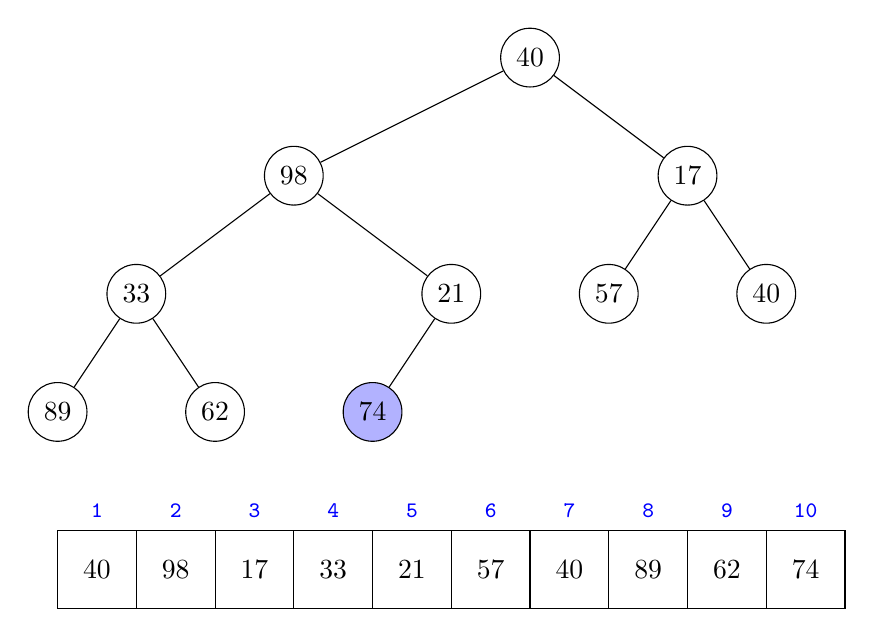
\begin{tikzpicture}
                % Sequência de inserção: 40, 98, 17, 33, 21, 57, 40, 89, 62, 74
                \node[circle,draw] (A) at (6, 6) { 40 };
                \node[circle,draw] (B) at (3, 4.5) { 98 };
                \node[circle,draw] (C) at (8, 4.5) { 17 };
                \node[circle,draw] (D) at (1, 3) { 33 };
                \node[circle,draw] (E) at (5, 3) { 21 };
                \node[circle,draw] (F) at (7, 3) { 57 };
                \node[circle,draw] (G) at (9, 3) { 40 };
                \node[circle,draw] (H) at (0, 1.5) { 89 };
                \node[circle,draw] (I) at (2, 1.5) { 62 };
                \node[circle,draw,fill=blue!30] (J) at (4, 1.5) { 74 };

                \draw (A) -- (B);
                \draw (A) -- (C);
                \draw (B) -- (D);
                \draw (B) -- (E);
                \draw (C) -- (F);
                \draw (C) -- (G);
                \draw (D) -- (H);
                \draw (D) -- (I);
                \draw (E) -- (J);

                \draw (0, -1) grid (10, 0);

                \node[color=blue] at (0.5, 0.25) { \footnotesize \texttt{\textbf{1}} };
                \node[color=blue] at (1.5, 0.25) { \footnotesize \texttt{\textbf{2}} };
                \node[color=blue] at (2.5, 0.25) { \footnotesize \texttt{\textbf{3}} };
                \node[color=blue] at (3.5, 0.25) { \footnotesize \texttt{\textbf{4}} };
                \node[color=blue] at (4.5, 0.25) { \footnotesize \texttt{\textbf{5}} };
                \node[color=blue] at (5.5, 0.25) { \footnotesize \texttt{\textbf{6}} };
                \node[color=blue] at (6.5, 0.25) { \footnotesize \texttt{\textbf{7}} };
                \node[color=blue] at (7.5, 0.25) { \footnotesize \texttt{\textbf{8}} };
                \node[color=blue] at (8.5, 0.25) { \footnotesize \texttt{\textbf{9}} };
                \node[color=blue] at (9.5, 0.25) { \footnotesize \texttt{\textbf{10}} };

                \node at (0.5, -0.5) { 40 };
                \node at (1.5, -0.5) { 98 };
                \node at (2.5, -0.5) { 17 };
                \node at (3.5, -0.5) { 33 };
                \node at (4.5, -0.5) { 21 };
                \node at (5.5, -0.5) { 57 };
                \node at (6.5, -0.5) { 40 };
                \node at (7.5, -0.5) { 89 };
                \node at (8.5, -0.5) { 62 };
                \node at (9.5, -0.5) { 74 };
        \end{tikzpicture}
    \end{figure}

\end{frame}

\begin{frame}[fragile]{Exemplo de execução da rotina \code{c}{heapify()}}

    \begin{figure}
        \centering
        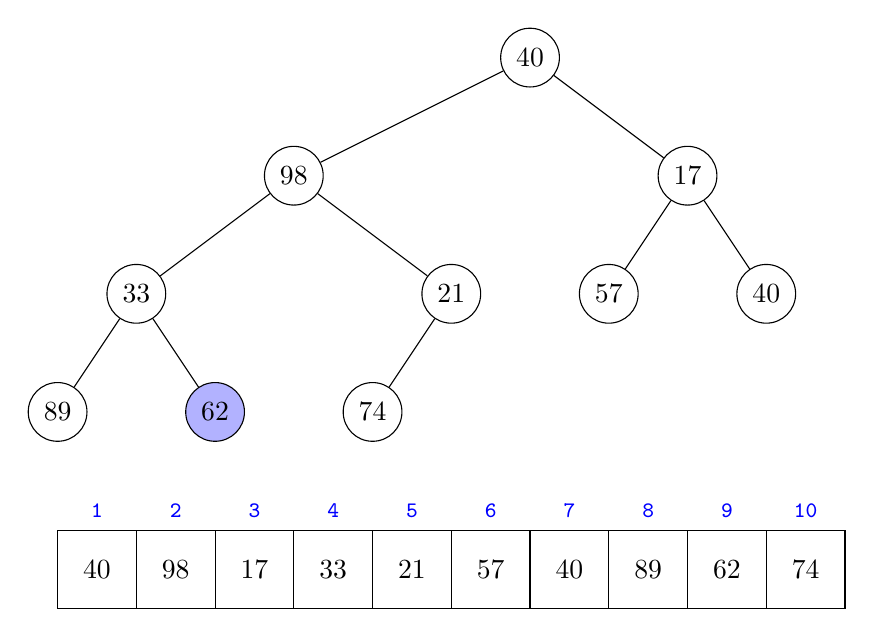
\begin{tikzpicture}
                % Sequência de inserção: 40, 98, 17, 33, 21, 57, 40, 89, 62, 74
                \node[circle,draw] (A) at (6, 6) { 40 };
                \node[circle,draw] (B) at (3, 4.5) { 98 };
                \node[circle,draw] (C) at (8, 4.5) { 17 };
                \node[circle,draw] (D) at (1, 3) { 33 };
                \node[circle,draw] (E) at (5, 3) { 21 };
                \node[circle,draw] (F) at (7, 3) { 57 };
                \node[circle,draw] (G) at (9, 3) { 40 };
                \node[circle,draw] (H) at (0, 1.5) { 89 };
                \node[circle,draw,fill=blue!30] (I) at (2, 1.5) { 62 };
                \node[circle,draw] (J) at (4, 1.5) { 74 };

                \draw (A) -- (B);
                \draw (A) -- (C);
                \draw (B) -- (D);
                \draw (B) -- (E);
                \draw (C) -- (F);
                \draw (C) -- (G);
                \draw (D) -- (H);
                \draw (D) -- (I);
                \draw (E) -- (J);

                \draw (0, -1) grid (10, 0);

                \node[color=blue] at (0.5, 0.25) { \footnotesize \texttt{\textbf{1}} };
                \node[color=blue] at (1.5, 0.25) { \footnotesize \texttt{\textbf{2}} };
                \node[color=blue] at (2.5, 0.25) { \footnotesize \texttt{\textbf{3}} };
                \node[color=blue] at (3.5, 0.25) { \footnotesize \texttt{\textbf{4}} };
                \node[color=blue] at (4.5, 0.25) { \footnotesize \texttt{\textbf{5}} };
                \node[color=blue] at (5.5, 0.25) { \footnotesize \texttt{\textbf{6}} };
                \node[color=blue] at (6.5, 0.25) { \footnotesize \texttt{\textbf{7}} };
                \node[color=blue] at (7.5, 0.25) { \footnotesize \texttt{\textbf{8}} };
                \node[color=blue] at (8.5, 0.25) { \footnotesize \texttt{\textbf{9}} };
                \node[color=blue] at (9.5, 0.25) { \footnotesize \texttt{\textbf{10}} };

                \node at (0.5, -0.5) { 40 };
                \node at (1.5, -0.5) { 98 };
                \node at (2.5, -0.5) { 17 };
                \node at (3.5, -0.5) { 33 };
                \node at (4.5, -0.5) { 21 };
                \node at (5.5, -0.5) { 57 };
                \node at (6.5, -0.5) { 40 };
                \node at (7.5, -0.5) { 89 };
                \node at (8.5, -0.5) { 62 };
                \node at (9.5, -0.5) { 74 };
        \end{tikzpicture}
    \end{figure}

\end{frame}

\begin{frame}[fragile]{Exemplo de execução da rotina \code{c}{heapify()}}

    \begin{figure}
        \centering
        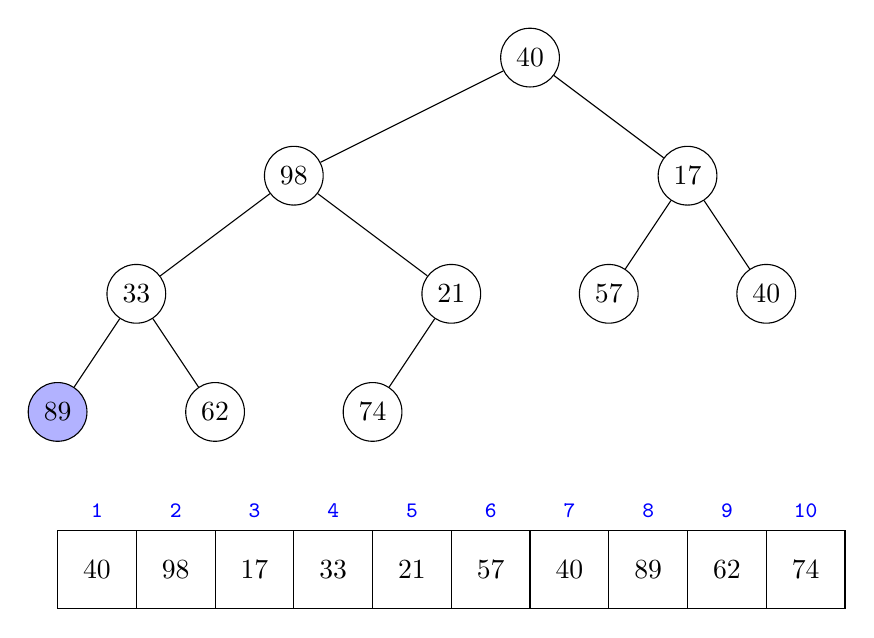
\begin{tikzpicture}
                % Sequência de inserção: 40, 98, 17, 33, 21, 57, 40, 89, 62, 74
                \node[circle,draw] (A) at (6, 6) { 40 };
                \node[circle,draw] (B) at (3, 4.5) { 98 };
                \node[circle,draw] (C) at (8, 4.5) { 17 };
                \node[circle,draw] (D) at (1, 3) { 33 };
                \node[circle,draw] (E) at (5, 3) { 21 };
                \node[circle,draw] (F) at (7, 3) { 57 };
                \node[circle,draw] (G) at (9, 3) { 40 };
                \node[circle,draw,fill=blue!30] (H) at (0, 1.5) { 89 };
                \node[circle,draw] (I) at (2, 1.5) { 62 };
                \node[circle,draw] (J) at (4, 1.5) { 74 };

                \draw (A) -- (B);
                \draw (A) -- (C);
                \draw (B) -- (D);
                \draw (B) -- (E);
                \draw (C) -- (F);
                \draw (C) -- (G);
                \draw (D) -- (H);
                \draw (D) -- (I);
                \draw (E) -- (J);

                \draw (0, -1) grid (10, 0);

                \node[color=blue] at (0.5, 0.25) { \footnotesize \texttt{\textbf{1}} };
                \node[color=blue] at (1.5, 0.25) { \footnotesize \texttt{\textbf{2}} };
                \node[color=blue] at (2.5, 0.25) { \footnotesize \texttt{\textbf{3}} };
                \node[color=blue] at (3.5, 0.25) { \footnotesize \texttt{\textbf{4}} };
                \node[color=blue] at (4.5, 0.25) { \footnotesize \texttt{\textbf{5}} };
                \node[color=blue] at (5.5, 0.25) { \footnotesize \texttt{\textbf{6}} };
                \node[color=blue] at (6.5, 0.25) { \footnotesize \texttt{\textbf{7}} };
                \node[color=blue] at (7.5, 0.25) { \footnotesize \texttt{\textbf{8}} };
                \node[color=blue] at (8.5, 0.25) { \footnotesize \texttt{\textbf{9}} };
                \node[color=blue] at (9.5, 0.25) { \footnotesize \texttt{\textbf{10}} };

                \node at (0.5, -0.5) { 40 };
                \node at (1.5, -0.5) { 98 };
                \node at (2.5, -0.5) { 17 };
                \node at (3.5, -0.5) { 33 };
                \node at (4.5, -0.5) { 21 };
                \node at (5.5, -0.5) { 57 };
                \node at (6.5, -0.5) { 40 };
                \node at (7.5, -0.5) { 89 };
                \node at (8.5, -0.5) { 62 };
                \node at (9.5, -0.5) { 74 };
        \end{tikzpicture}
    \end{figure}

\end{frame}

\begin{frame}[fragile]{Exemplo de execução da rotina \code{c}{heapify()}}

    \begin{figure}
        \centering
        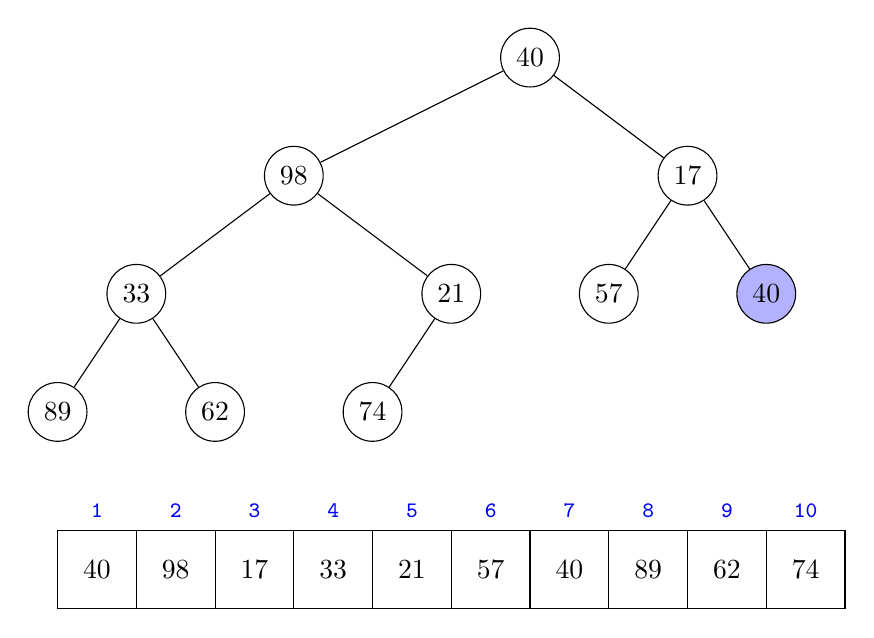
\begin{tikzpicture}
                % Sequência de inserção: 40, 98, 17, 33, 21, 57, 40, 89, 62, 74
                \node[circle,draw] (A) at (6, 6) { 40 };
                \node[circle,draw] (B) at (3, 4.5) { 98 };
                \node[circle,draw] (C) at (8, 4.5) { 17 };
                \node[circle,draw] (D) at (1, 3) { 33 };
                \node[circle,draw] (E) at (5, 3) { 21 };
                \node[circle,draw] (F) at (7, 3) { 57 };
                \node[circle,draw,fill=blue!30] (G) at (9, 3) { 40 };
                \node[circle,draw] (H) at (0, 1.5) { 89 };
                \node[circle,draw] (I) at (2, 1.5) { 62 };
                \node[circle,draw] (J) at (4, 1.5) { 74 };

                \draw (A) -- (B);
                \draw (A) -- (C);
                \draw (B) -- (D);
                \draw (B) -- (E);
                \draw (C) -- (F);
                \draw (C) -- (G);
                \draw (D) -- (H);
                \draw (D) -- (I);
                \draw (E) -- (J);

                \draw (0, -1) grid (10, 0);

                \node[color=blue] at (0.5, 0.25) { \footnotesize \texttt{\textbf{1}} };
                \node[color=blue] at (1.5, 0.25) { \footnotesize \texttt{\textbf{2}} };
                \node[color=blue] at (2.5, 0.25) { \footnotesize \texttt{\textbf{3}} };
                \node[color=blue] at (3.5, 0.25) { \footnotesize \texttt{\textbf{4}} };
                \node[color=blue] at (4.5, 0.25) { \footnotesize \texttt{\textbf{5}} };
                \node[color=blue] at (5.5, 0.25) { \footnotesize \texttt{\textbf{6}} };
                \node[color=blue] at (6.5, 0.25) { \footnotesize \texttt{\textbf{7}} };
                \node[color=blue] at (7.5, 0.25) { \footnotesize \texttt{\textbf{8}} };
                \node[color=blue] at (8.5, 0.25) { \footnotesize \texttt{\textbf{9}} };
                \node[color=blue] at (9.5, 0.25) { \footnotesize \texttt{\textbf{10}} };

                \node at (0.5, -0.5) { 40 };
                \node at (1.5, -0.5) { 98 };
                \node at (2.5, -0.5) { 17 };
                \node at (3.5, -0.5) { 33 };
                \node at (4.5, -0.5) { 21 };
                \node at (5.5, -0.5) { 57 };
                \node at (6.5, -0.5) { 40 };
                \node at (7.5, -0.5) { 89 };
                \node at (8.5, -0.5) { 62 };
                \node at (9.5, -0.5) { 74 };
        \end{tikzpicture}
    \end{figure}

\end{frame}

\begin{frame}[fragile]{Exemplo de execução da rotina \code{c}{heapify()}}

    \begin{figure}
        \centering
        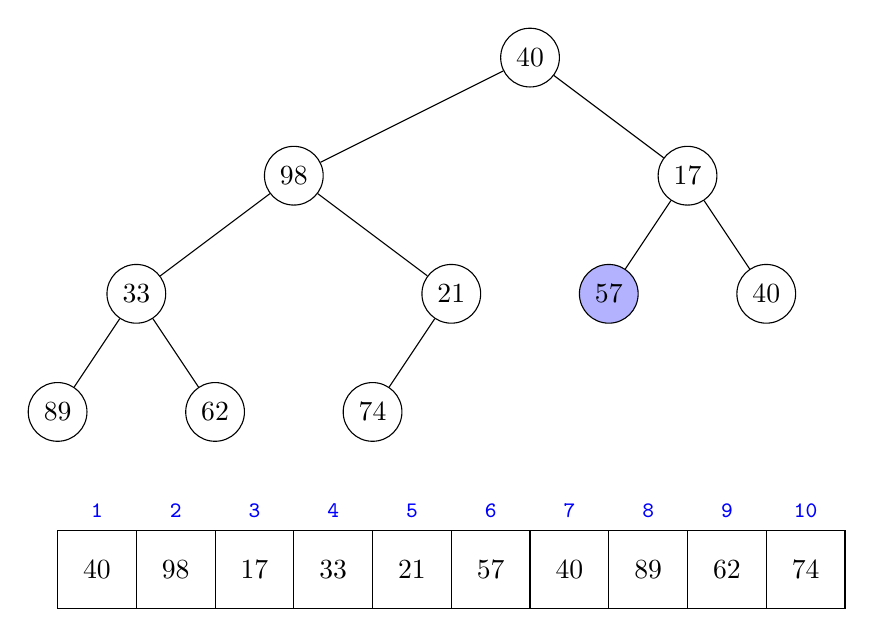
\begin{tikzpicture}
                % Sequência de inserção: 40, 98, 17, 33, 21, 57, 40, 89, 62, 74
                \node[circle,draw] (A) at (6, 6) { 40 };
                \node[circle,draw] (B) at (3, 4.5) { 98 };
                \node[circle,draw] (C) at (8, 4.5) { 17 };
                \node[circle,draw] (D) at (1, 3) { 33 };
                \node[circle,draw] (E) at (5, 3) { 21 };
                \node[circle,draw,fill=blue!30] (F) at (7, 3) { 57 };
                \node[circle,draw] (G) at (9, 3) { 40 };
                \node[circle,draw] (H) at (0, 1.5) { 89 };
                \node[circle,draw] (I) at (2, 1.5) { 62 };
                \node[circle,draw] (J) at (4, 1.5) { 74 };

                \draw (A) -- (B);
                \draw (A) -- (C);
                \draw (B) -- (D);
                \draw (B) -- (E);
                \draw (C) -- (F);
                \draw (C) -- (G);
                \draw (D) -- (H);
                \draw (D) -- (I);
                \draw (E) -- (J);

                \draw (0, -1) grid (10, 0);

                \node[color=blue] at (0.5, 0.25) { \footnotesize \texttt{\textbf{1}} };
                \node[color=blue] at (1.5, 0.25) { \footnotesize \texttt{\textbf{2}} };
                \node[color=blue] at (2.5, 0.25) { \footnotesize \texttt{\textbf{3}} };
                \node[color=blue] at (3.5, 0.25) { \footnotesize \texttt{\textbf{4}} };
                \node[color=blue] at (4.5, 0.25) { \footnotesize \texttt{\textbf{5}} };
                \node[color=blue] at (5.5, 0.25) { \footnotesize \texttt{\textbf{6}} };
                \node[color=blue] at (6.5, 0.25) { \footnotesize \texttt{\textbf{7}} };
                \node[color=blue] at (7.5, 0.25) { \footnotesize \texttt{\textbf{8}} };
                \node[color=blue] at (8.5, 0.25) { \footnotesize \texttt{\textbf{9}} };
                \node[color=blue] at (9.5, 0.25) { \footnotesize \texttt{\textbf{10}} };

                \node at (0.5, -0.5) { 40 };
                \node at (1.5, -0.5) { 98 };
                \node at (2.5, -0.5) { 17 };
                \node at (3.5, -0.5) { 33 };
                \node at (4.5, -0.5) { 21 };
                \node at (5.5, -0.5) { 57 };
                \node at (6.5, -0.5) { 40 };
                \node at (7.5, -0.5) { 89 };
                \node at (8.5, -0.5) { 62 };
                \node at (9.5, -0.5) { 74 };
        \end{tikzpicture}
    \end{figure}

\end{frame}

\begin{frame}[fragile]{Exemplo de execução da rotina \code{c}{heapify()}}

    \begin{figure}
        \centering
        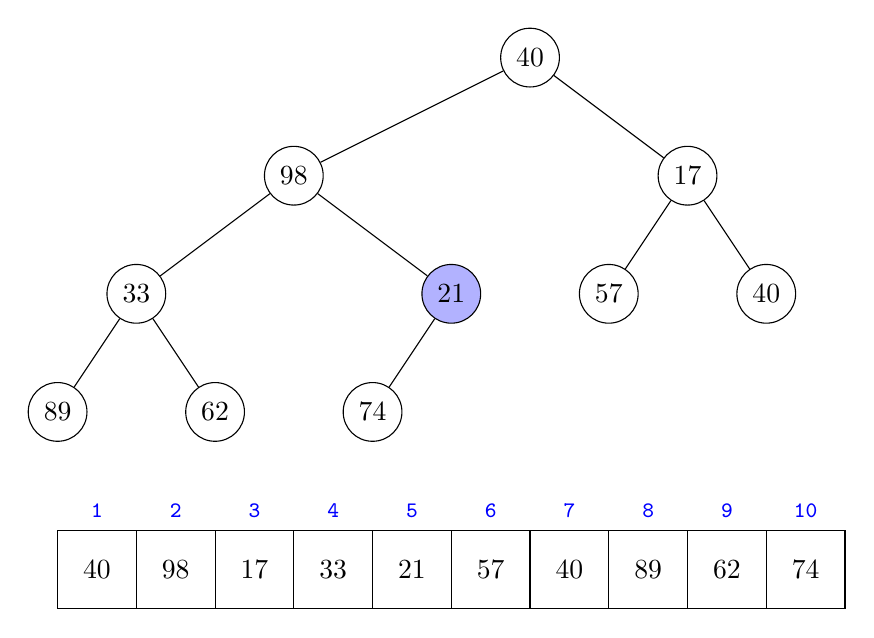
\begin{tikzpicture}
                % Sequência de inserção: 40, 98, 17, 33, 21, 57, 40, 89, 62, 74
                \node[circle,draw] (A) at (6, 6) { 40 };
                \node[circle,draw] (B) at (3, 4.5) { 98 };
                \node[circle,draw] (C) at (8, 4.5) { 17 };
                \node[circle,draw] (D) at (1, 3) { 33 };
                \node[circle,draw,fill=blue!30] (E) at (5, 3) { 21 };
                \node[circle,draw] (F) at (7, 3) { 57 };
                \node[circle,draw] (G) at (9, 3) { 40 };
                \node[circle,draw] (H) at (0, 1.5) { 89 };
                \node[circle,draw] (I) at (2, 1.5) { 62 };
                \node[circle,draw] (J) at (4, 1.5) { 74 };

                \draw (A) -- (B);
                \draw (A) -- (C);
                \draw (B) -- (D);
                \draw (B) -- (E);
                \draw (C) -- (F);
                \draw (C) -- (G);
                \draw (D) -- (H);
                \draw (D) -- (I);
                \draw (E) -- (J);

                \draw (0, -1) grid (10, 0);

                \node[color=blue] at (0.5, 0.25) { \footnotesize \texttt{\textbf{1}} };
                \node[color=blue] at (1.5, 0.25) { \footnotesize \texttt{\textbf{2}} };
                \node[color=blue] at (2.5, 0.25) { \footnotesize \texttt{\textbf{3}} };
                \node[color=blue] at (3.5, 0.25) { \footnotesize \texttt{\textbf{4}} };
                \node[color=blue] at (4.5, 0.25) { \footnotesize \texttt{\textbf{5}} };
                \node[color=blue] at (5.5, 0.25) { \footnotesize \texttt{\textbf{6}} };
                \node[color=blue] at (6.5, 0.25) { \footnotesize \texttt{\textbf{7}} };
                \node[color=blue] at (7.5, 0.25) { \footnotesize \texttt{\textbf{8}} };
                \node[color=blue] at (8.5, 0.25) { \footnotesize \texttt{\textbf{9}} };
                \node[color=blue] at (9.5, 0.25) { \footnotesize \texttt{\textbf{10}} };

                \node at (0.5, -0.5) { 40 };
                \node at (1.5, -0.5) { 98 };
                \node at (2.5, -0.5) { 17 };
                \node at (3.5, -0.5) { 33 };
                \node at (4.5, -0.5) { 21 };
                \node at (5.5, -0.5) { 57 };
                \node at (6.5, -0.5) { 40 };
                \node at (7.5, -0.5) { 89 };
                \node at (8.5, -0.5) { 62 };
                \node at (9.5, -0.5) { 74 };
        \end{tikzpicture}
    \end{figure}

\end{frame}

\begin{frame}[fragile]{Exemplo de execução da rotina \code{c}{heapify()}}

    \begin{figure}
        \centering
        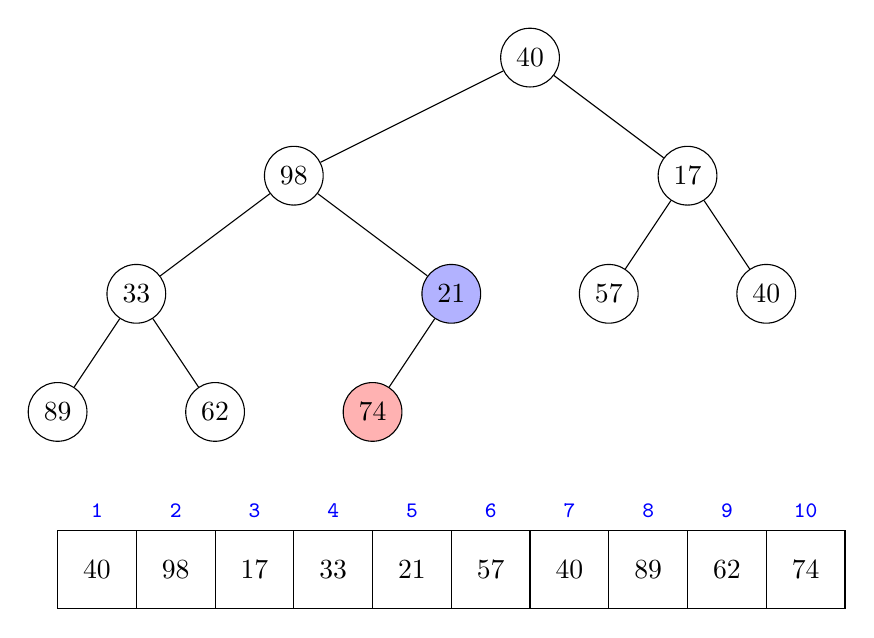
\begin{tikzpicture}
                % Sequência de inserção: 40, 98, 17, 33, 21, 57, 40, 89, 62, 74
                \node[circle,draw] (A) at (6, 6) { 40 };
                \node[circle,draw] (B) at (3, 4.5) { 98 };
                \node[circle,draw] (C) at (8, 4.5) { 17 };
                \node[circle,draw] (D) at (1, 3) { 33 };
                \node[circle,draw,fill=blue!30] (E) at (5, 3) { 21 };
                \node[circle,draw] (F) at (7, 3) { 57 };
                \node[circle,draw] (G) at (9, 3) { 40 };
                \node[circle,draw] (H) at (0, 1.5) { 89 };
                \node[circle,draw] (I) at (2, 1.5) { 62 };
                \node[circle,draw,fill=red!30] (J) at (4, 1.5) { 74 };

                \draw (A) -- (B);
                \draw (A) -- (C);
                \draw (B) -- (D);
                \draw (B) -- (E);
                \draw (C) -- (F);
                \draw (C) -- (G);
                \draw (D) -- (H);
                \draw (D) -- (I);
                \draw (E) -- (J);

                \draw (0, -1) grid (10, 0);

                \node[color=blue] at (0.5, 0.25) { \footnotesize \texttt{\textbf{1}} };
                \node[color=blue] at (1.5, 0.25) { \footnotesize \texttt{\textbf{2}} };
                \node[color=blue] at (2.5, 0.25) { \footnotesize \texttt{\textbf{3}} };
                \node[color=blue] at (3.5, 0.25) { \footnotesize \texttt{\textbf{4}} };
                \node[color=blue] at (4.5, 0.25) { \footnotesize \texttt{\textbf{5}} };
                \node[color=blue] at (5.5, 0.25) { \footnotesize \texttt{\textbf{6}} };
                \node[color=blue] at (6.5, 0.25) { \footnotesize \texttt{\textbf{7}} };
                \node[color=blue] at (7.5, 0.25) { \footnotesize \texttt{\textbf{8}} };
                \node[color=blue] at (8.5, 0.25) { \footnotesize \texttt{\textbf{9}} };
                \node[color=blue] at (9.5, 0.25) { \footnotesize \texttt{\textbf{10}} };

                \node at (0.5, -0.5) { 40 };
                \node at (1.5, -0.5) { 98 };
                \node at (2.5, -0.5) { 17 };
                \node at (3.5, -0.5) { 33 };
                \node at (4.5, -0.5) { 21 };
                \node at (5.5, -0.5) { 57 };
                \node at (6.5, -0.5) { 40 };
                \node at (7.5, -0.5) { 89 };
                \node at (8.5, -0.5) { 62 };
                \node at (9.5, -0.5) { 74 };
        \end{tikzpicture}
    \end{figure}

\end{frame}

\begin{frame}[fragile]{Exemplo de execução da rotina \code{c}{heapify()}}

    \begin{figure}
        \centering
        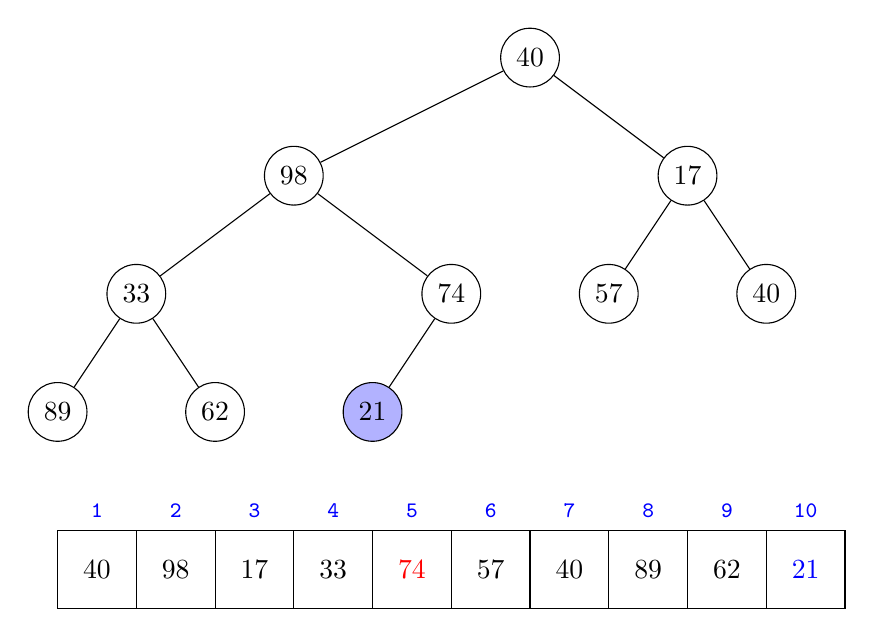
\begin{tikzpicture}
                % Sequência de inserção: 40, 98, 17, 33, 21, 57, 40, 89, 62, 74
                \node[circle,draw] (A) at (6, 6) { 40 };
                \node[circle,draw] (B) at (3, 4.5) { 98 };
                \node[circle,draw] (C) at (8, 4.5) { 17 };
                \node[circle,draw] (D) at (1, 3) { 33 };
                \node[circle,draw] (E) at (5, 3) { 74 };
                \node[circle,draw] (F) at (7, 3) { 57 };
                \node[circle,draw] (G) at (9, 3) { 40 };
                \node[circle,draw] (H) at (0, 1.5) { 89 };
                \node[circle,draw] (I) at (2, 1.5) { 62 };
                \node[circle,draw,fill=blue!30] (J) at (4, 1.5) { 21 };

                \draw (A) -- (B);
                \draw (A) -- (C);
                \draw (B) -- (D);
                \draw (B) -- (E);
                \draw (C) -- (F);
                \draw (C) -- (G);
                \draw (D) -- (H);
                \draw (D) -- (I);
                \draw (E) -- (J);

                \draw (0, -1) grid (10, 0);

                \node[color=blue] at (0.5, 0.25) { \footnotesize \texttt{\textbf{1}} };
                \node[color=blue] at (1.5, 0.25) { \footnotesize \texttt{\textbf{2}} };
                \node[color=blue] at (2.5, 0.25) { \footnotesize \texttt{\textbf{3}} };
                \node[color=blue] at (3.5, 0.25) { \footnotesize \texttt{\textbf{4}} };
                \node[color=blue] at (4.5, 0.25) { \footnotesize \texttt{\textbf{5}} };
                \node[color=blue] at (5.5, 0.25) { \footnotesize \texttt{\textbf{6}} };
                \node[color=blue] at (6.5, 0.25) { \footnotesize \texttt{\textbf{7}} };
                \node[color=blue] at (7.5, 0.25) { \footnotesize \texttt{\textbf{8}} };
                \node[color=blue] at (8.5, 0.25) { \footnotesize \texttt{\textbf{9}} };
                \node[color=blue] at (9.5, 0.25) { \footnotesize \texttt{\textbf{10}} };

                \node at (0.5, -0.5) { 40 };
                \node at (1.5, -0.5) { 98 };
                \node at (2.5, -0.5) { 17 };
                \node at (3.5, -0.5) { 33 };
                \node at (4.5, -0.5) { \textcolor{red}{74} };
                \node at (5.5, -0.5) { 57 };
                \node at (6.5, -0.5) { 40 };
                \node at (7.5, -0.5) { 89 };
                \node at (8.5, -0.5) { 62 };
                \node at (9.5, -0.5) { \textcolor{blue}{21} };
        \end{tikzpicture}
    \end{figure}

\end{frame}

\begin{frame}[fragile]{Exemplo de execução da rotina \code{c}{heapify()}}

    \begin{figure}
        \centering
        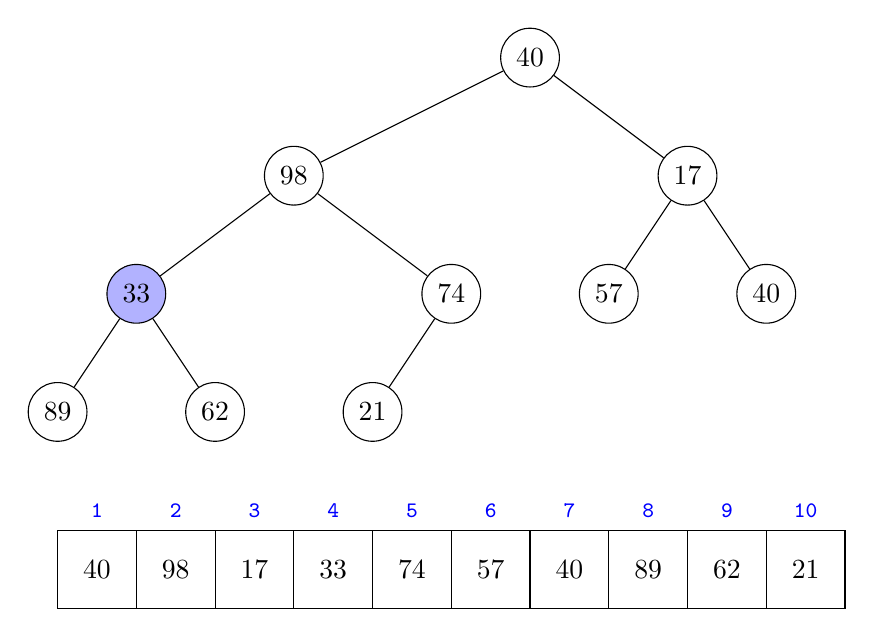
\begin{tikzpicture}
                % Sequência de inserção: 40, 98, 17, 33, 21, 57, 40, 89, 62, 74
                \node[circle,draw] (A) at (6, 6) { 40 };
                \node[circle,draw] (B) at (3, 4.5) { 98 };
                \node[circle,draw] (C) at (8, 4.5) { 17 };
                \node[circle,draw,fill=blue!30] (D) at (1, 3) { 33 };
                \node[circle,draw] (E) at (5, 3) { 74 };
                \node[circle,draw] (F) at (7, 3) { 57 };
                \node[circle,draw] (G) at (9, 3) { 40 };
                \node[circle,draw] (H) at (0, 1.5) { 89 };
                \node[circle,draw] (I) at (2, 1.5) { 62 };
                \node[circle,draw] (J) at (4, 1.5) { 21 };

                \draw (A) -- (B);
                \draw (A) -- (C);
                \draw (B) -- (D);
                \draw (B) -- (E);
                \draw (C) -- (F);
                \draw (C) -- (G);
                \draw (D) -- (H);
                \draw (D) -- (I);
                \draw (E) -- (J);

                \draw (0, -1) grid (10, 0);

                \node[color=blue] at (0.5, 0.25) { \footnotesize \texttt{\textbf{1}} };
                \node[color=blue] at (1.5, 0.25) { \footnotesize \texttt{\textbf{2}} };
                \node[color=blue] at (2.5, 0.25) { \footnotesize \texttt{\textbf{3}} };
                \node[color=blue] at (3.5, 0.25) { \footnotesize \texttt{\textbf{4}} };
                \node[color=blue] at (4.5, 0.25) { \footnotesize \texttt{\textbf{5}} };
                \node[color=blue] at (5.5, 0.25) { \footnotesize \texttt{\textbf{6}} };
                \node[color=blue] at (6.5, 0.25) { \footnotesize \texttt{\textbf{7}} };
                \node[color=blue] at (7.5, 0.25) { \footnotesize \texttt{\textbf{8}} };
                \node[color=blue] at (8.5, 0.25) { \footnotesize \texttt{\textbf{9}} };
                \node[color=blue] at (9.5, 0.25) { \footnotesize \texttt{\textbf{10}} };

                \node at (0.5, -0.5) { 40 };
                \node at (1.5, -0.5) { 98 };
                \node at (2.5, -0.5) { 17 };
                \node at (3.5, -0.5) { 33 };
                \node at (4.5, -0.5) { \textcolor{black}{74} };
                \node at (5.5, -0.5) { 57 };
                \node at (6.5, -0.5) { 40 };
                \node at (7.5, -0.5) { 89 };
                \node at (8.5, -0.5) { 62 };
                \node at (9.5, -0.5) { \textcolor{black}{21} };
        \end{tikzpicture}
    \end{figure}

\end{frame}

\begin{frame}[fragile]{Exemplo de execução da rotina \code{c}{heapify()}}

    \begin{figure}
        \centering
        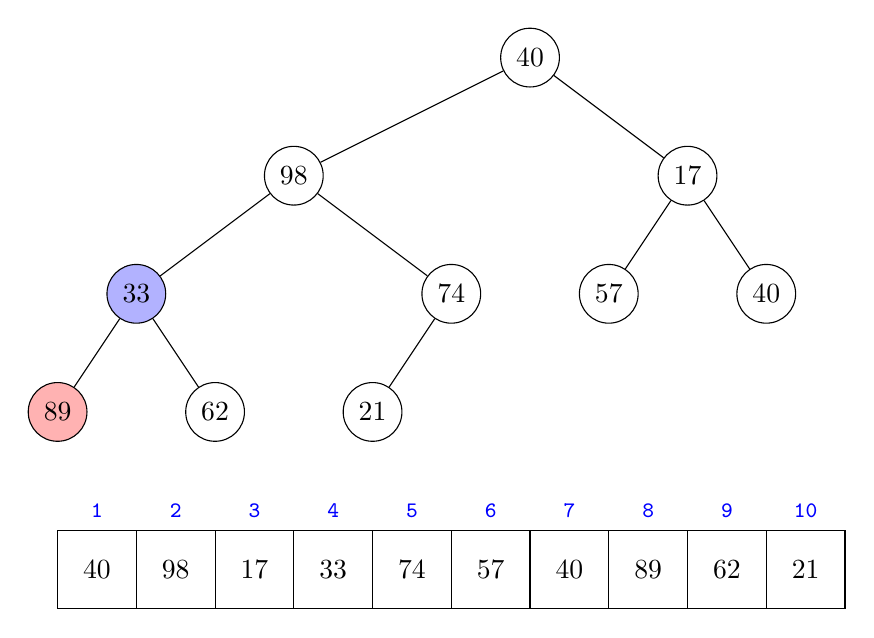
\begin{tikzpicture}
                % Sequência de inserção: 40, 98, 17, 33, 21, 57, 40, 89, 62, 74
                \node[circle,draw] (A) at (6, 6) { 40 };
                \node[circle,draw] (B) at (3, 4.5) { 98 };
                \node[circle,draw] (C) at (8, 4.5) { 17 };
                \node[circle,draw,fill=blue!30] (D) at (1, 3) { 33 };
                \node[circle,draw] (E) at (5, 3) { 74 };
                \node[circle,draw] (F) at (7, 3) { 57 };
                \node[circle,draw] (G) at (9, 3) { 40 };
                \node[circle,draw,fill=red!30] (H) at (0, 1.5) { 89 };
                \node[circle,draw] (I) at (2, 1.5) { 62 };
                \node[circle,draw] (J) at (4, 1.5) { 21 };

                \draw (A) -- (B);
                \draw (A) -- (C);
                \draw (B) -- (D);
                \draw (B) -- (E);
                \draw (C) -- (F);
                \draw (C) -- (G);
                \draw (D) -- (H);
                \draw (D) -- (I);
                \draw (E) -- (J);

                \draw (0, -1) grid (10, 0);

                \node[color=blue] at (0.5, 0.25) { \footnotesize \texttt{\textbf{1}} };
                \node[color=blue] at (1.5, 0.25) { \footnotesize \texttt{\textbf{2}} };
                \node[color=blue] at (2.5, 0.25) { \footnotesize \texttt{\textbf{3}} };
                \node[color=blue] at (3.5, 0.25) { \footnotesize \texttt{\textbf{4}} };
                \node[color=blue] at (4.5, 0.25) { \footnotesize \texttt{\textbf{5}} };
                \node[color=blue] at (5.5, 0.25) { \footnotesize \texttt{\textbf{6}} };
                \node[color=blue] at (6.5, 0.25) { \footnotesize \texttt{\textbf{7}} };
                \node[color=blue] at (7.5, 0.25) { \footnotesize \texttt{\textbf{8}} };
                \node[color=blue] at (8.5, 0.25) { \footnotesize \texttt{\textbf{9}} };
                \node[color=blue] at (9.5, 0.25) { \footnotesize \texttt{\textbf{10}} };

                \node at (0.5, -0.5) { 40 };
                \node at (1.5, -0.5) { 98 };
                \node at (2.5, -0.5) { 17 };
                \node at (3.5, -0.5) { 33 };
                \node at (4.5, -0.5) { \textcolor{black}{74} };
                \node at (5.5, -0.5) { 57 };
                \node at (6.5, -0.5) { 40 };
                \node at (7.5, -0.5) { 89 };
                \node at (8.5, -0.5) { 62 };
                \node at (9.5, -0.5) { \textcolor{black}{21} };
        \end{tikzpicture}
    \end{figure}

\end{frame}

\begin{frame}[fragile]{Exemplo de execução da rotina \code{c}{heapify()}}

    \begin{figure}
        \centering
        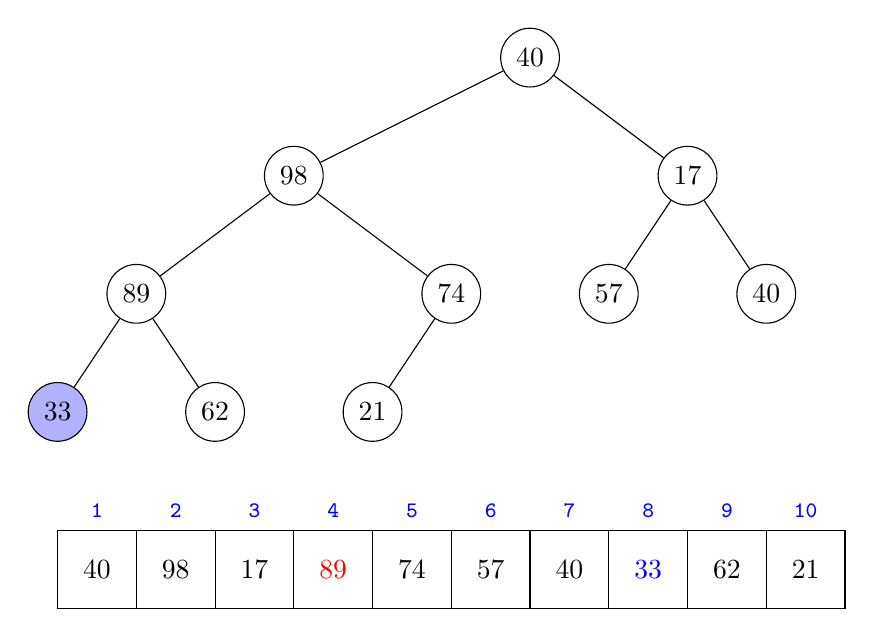
\begin{tikzpicture}
                % Sequência de inserção: 40, 98, 17, 33, 21, 57, 40, 89, 62, 74
                \node[circle,draw] (A) at (6, 6) { 40 };
                \node[circle,draw] (B) at (3, 4.5) { 98 };
                \node[circle,draw] (C) at (8, 4.5) { 17 };
                \node[circle,draw] (D) at (1, 3) { 89 };
                \node[circle,draw] (E) at (5, 3) { 74 };
                \node[circle,draw] (F) at (7, 3) { 57 };
                \node[circle,draw] (G) at (9, 3) { 40 };
                \node[circle,draw,fill=blue!30] (H) at (0, 1.5) { 33 };
                \node[circle,draw] (I) at (2, 1.5) { 62 };
                \node[circle,draw] (J) at (4, 1.5) { 21 };

                \draw (A) -- (B);
                \draw (A) -- (C);
                \draw (B) -- (D);
                \draw (B) -- (E);
                \draw (C) -- (F);
                \draw (C) -- (G);
                \draw (D) -- (H);
                \draw (D) -- (I);
                \draw (E) -- (J);

                \draw (0, -1) grid (10, 0);

                \node[color=blue] at (0.5, 0.25) { \footnotesize \texttt{\textbf{1}} };
                \node[color=blue] at (1.5, 0.25) { \footnotesize \texttt{\textbf{2}} };
                \node[color=blue] at (2.5, 0.25) { \footnotesize \texttt{\textbf{3}} };
                \node[color=blue] at (3.5, 0.25) { \footnotesize \texttt{\textbf{4}} };
                \node[color=blue] at (4.5, 0.25) { \footnotesize \texttt{\textbf{5}} };
                \node[color=blue] at (5.5, 0.25) { \footnotesize \texttt{\textbf{6}} };
                \node[color=blue] at (6.5, 0.25) { \footnotesize \texttt{\textbf{7}} };
                \node[color=blue] at (7.5, 0.25) { \footnotesize \texttt{\textbf{8}} };
                \node[color=blue] at (8.5, 0.25) { \footnotesize \texttt{\textbf{9}} };
                \node[color=blue] at (9.5, 0.25) { \footnotesize \texttt{\textbf{10}} };

                \node at (0.5, -0.5) { 40 };
                \node at (1.5, -0.5) { 98 };
                \node at (2.5, -0.5) { 17 };
                \node at (3.5, -0.5) { \textcolor{red}{89} };
                \node at (4.5, -0.5) { \textcolor{black}{74} };
                \node at (5.5, -0.5) { 57 };
                \node at (6.5, -0.5) { 40 };
                \node at (7.5, -0.5) { \textcolor{blue}{33}};
                \node at (8.5, -0.5) { 62 };
                \node at (9.5, -0.5) { \textcolor{black}{21} };
        \end{tikzpicture}
    \end{figure}

\end{frame}

\begin{frame}[fragile]{Exemplo de execução da rotina \code{c}{heapify()}}

    \begin{figure}
        \centering
        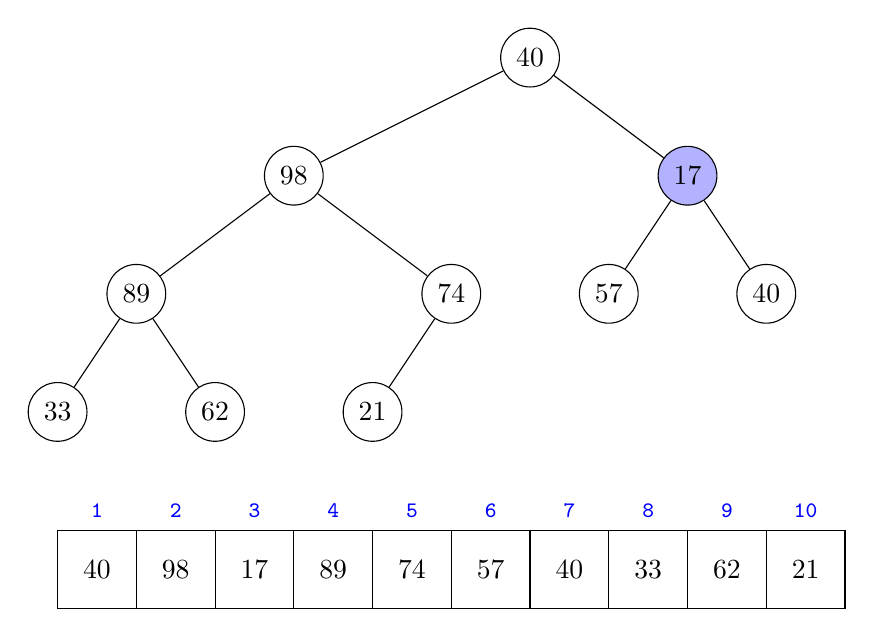
\begin{tikzpicture}
                % Sequência de inserção: 40, 98, 17, 33, 21, 57, 40, 89, 62, 74
                \node[circle,draw] (A) at (6, 6) { 40 };
                \node[circle,draw] (B) at (3, 4.5) { 98 };
                \node[circle,draw,fill=blue!30] (C) at (8, 4.5) { 17 };
                \node[circle,draw] (D) at (1, 3) { 89 };
                \node[circle,draw] (E) at (5, 3) { 74 };
                \node[circle,draw] (F) at (7, 3) { 57 };
                \node[circle,draw] (G) at (9, 3) { 40 };
                \node[circle,draw] (H) at (0, 1.5) { 33 };
                \node[circle,draw] (I) at (2, 1.5) { 62 };
                \node[circle,draw] (J) at (4, 1.5) { 21 };

                \draw (A) -- (B);
                \draw (A) -- (C);
                \draw (B) -- (D);
                \draw (B) -- (E);
                \draw (C) -- (F);
                \draw (C) -- (G);
                \draw (D) -- (H);
                \draw (D) -- (I);
                \draw (E) -- (J);

                \draw (0, -1) grid (10, 0);

                \node[color=blue] at (0.5, 0.25) { \footnotesize \texttt{\textbf{1}} };
                \node[color=blue] at (1.5, 0.25) { \footnotesize \texttt{\textbf{2}} };
                \node[color=blue] at (2.5, 0.25) { \footnotesize \texttt{\textbf{3}} };
                \node[color=blue] at (3.5, 0.25) { \footnotesize \texttt{\textbf{4}} };
                \node[color=blue] at (4.5, 0.25) { \footnotesize \texttt{\textbf{5}} };
                \node[color=blue] at (5.5, 0.25) { \footnotesize \texttt{\textbf{6}} };
                \node[color=blue] at (6.5, 0.25) { \footnotesize \texttt{\textbf{7}} };
                \node[color=blue] at (7.5, 0.25) { \footnotesize \texttt{\textbf{8}} };
                \node[color=blue] at (8.5, 0.25) { \footnotesize \texttt{\textbf{9}} };
                \node[color=blue] at (9.5, 0.25) { \footnotesize \texttt{\textbf{10}} };

                \node at (0.5, -0.5) { 40 };
                \node at (1.5, -0.5) { 98 };
                \node at (2.5, -0.5) { 17 };
                \node at (3.5, -0.5) { \textcolor{black}{89} };
                \node at (4.5, -0.5) { \textcolor{black}{74} };
                \node at (5.5, -0.5) { 57 };
                \node at (6.5, -0.5) { 40 };
                \node at (7.5, -0.5) { \textcolor{black}{33}};
                \node at (8.5, -0.5) { 62 };
                \node at (9.5, -0.5) { \textcolor{black}{21} };
        \end{tikzpicture}
    \end{figure}

\end{frame}

\begin{frame}[fragile]{Exemplo de execução da rotina \code{c}{heapify()}}

    \begin{figure}
        \centering
        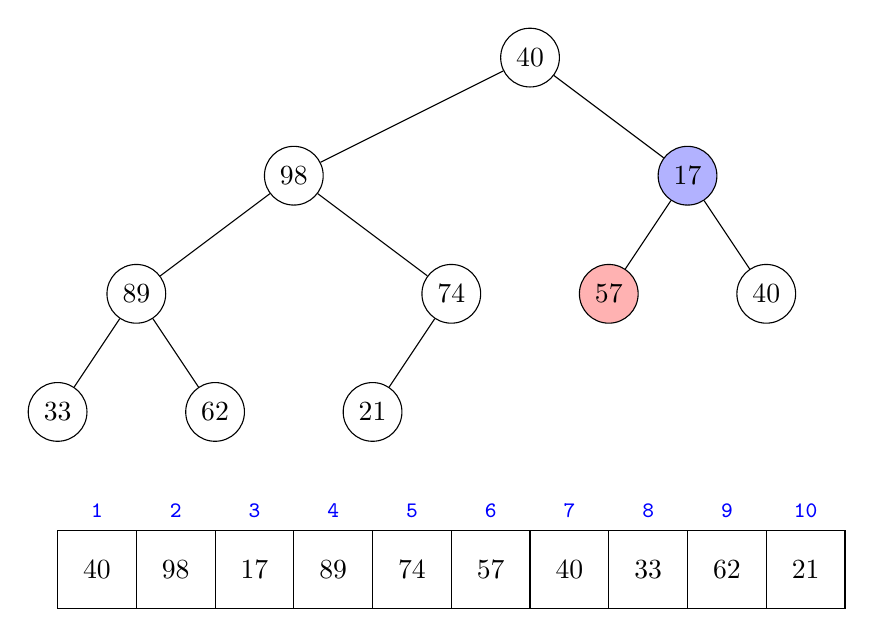
\begin{tikzpicture}
                % Sequência de inserção: 40, 98, 17, 33, 21, 57, 40, 89, 62, 74
                \node[circle,draw] (A) at (6, 6) { 40 };
                \node[circle,draw] (B) at (3, 4.5) { 98 };
                \node[circle,draw,fill=blue!30] (C) at (8, 4.5) { 17 };
                \node[circle,draw] (D) at (1, 3) { 89 };
                \node[circle,draw] (E) at (5, 3) { 74 };
                \node[circle,draw,fill=red!30] (F) at (7, 3) { 57 };
                \node[circle,draw] (G) at (9, 3) { 40 };
                \node[circle,draw] (H) at (0, 1.5) { 33 };
                \node[circle,draw] (I) at (2, 1.5) { 62 };
                \node[circle,draw] (J) at (4, 1.5) { 21 };

                \draw (A) -- (B);
                \draw (A) -- (C);
                \draw (B) -- (D);
                \draw (B) -- (E);
                \draw (C) -- (F);
                \draw (C) -- (G);
                \draw (D) -- (H);
                \draw (D) -- (I);
                \draw (E) -- (J);

                \draw (0, -1) grid (10, 0);

                \node[color=blue] at (0.5, 0.25) { \footnotesize \texttt{\textbf{1}} };
                \node[color=blue] at (1.5, 0.25) { \footnotesize \texttt{\textbf{2}} };
                \node[color=blue] at (2.5, 0.25) { \footnotesize \texttt{\textbf{3}} };
                \node[color=blue] at (3.5, 0.25) { \footnotesize \texttt{\textbf{4}} };
                \node[color=blue] at (4.5, 0.25) { \footnotesize \texttt{\textbf{5}} };
                \node[color=blue] at (5.5, 0.25) { \footnotesize \texttt{\textbf{6}} };
                \node[color=blue] at (6.5, 0.25) { \footnotesize \texttt{\textbf{7}} };
                \node[color=blue] at (7.5, 0.25) { \footnotesize \texttt{\textbf{8}} };
                \node[color=blue] at (8.5, 0.25) { \footnotesize \texttt{\textbf{9}} };
                \node[color=blue] at (9.5, 0.25) { \footnotesize \texttt{\textbf{10}} };

                \node at (0.5, -0.5) { 40 };
                \node at (1.5, -0.5) { 98 };
                \node at (2.5, -0.5) { 17 };
                \node at (3.5, -0.5) { \textcolor{black}{89} };
                \node at (4.5, -0.5) { \textcolor{black}{74} };
                \node at (5.5, -0.5) { 57 };
                \node at (6.5, -0.5) { 40 };
                \node at (7.5, -0.5) { \textcolor{black}{33}};
                \node at (8.5, -0.5) { 62 };
                \node at (9.5, -0.5) { \textcolor{black}{21} };
        \end{tikzpicture}
    \end{figure}

\end{frame}

\begin{frame}[fragile]{Exemplo de execução da rotina \code{c}{heapify()}}

    \begin{figure}
        \centering
        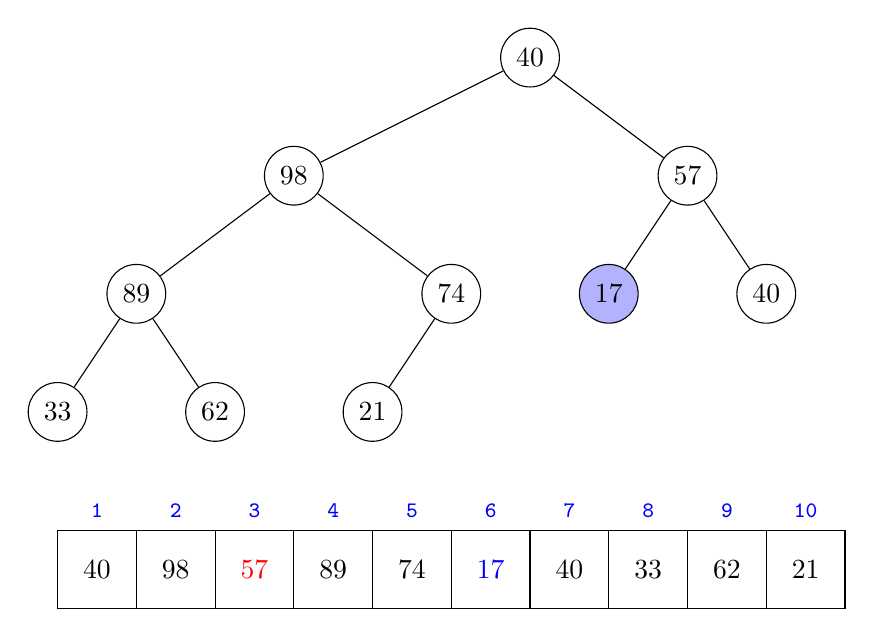
\begin{tikzpicture}
                % Sequência de inserção: 40, 98, 17, 33, 21, 57, 40, 89, 62, 74
                \node[circle,draw] (A) at (6, 6) { 40 };
                \node[circle,draw] (B) at (3, 4.5) { 98 };
                \node[circle,draw] (C) at (8, 4.5) { 57 };
                \node[circle,draw] (D) at (1, 3) { 89 };
                \node[circle,draw] (E) at (5, 3) { 74 };
                \node[circle,draw,fill=blue!30] (F) at (7, 3) { 17 };
                \node[circle,draw] (G) at (9, 3) { 40 };
                \node[circle,draw] (H) at (0, 1.5) { 33 };
                \node[circle,draw] (I) at (2, 1.5) { 62 };
                \node[circle,draw] (J) at (4, 1.5) { 21 };

                \draw (A) -- (B);
                \draw (A) -- (C);
                \draw (B) -- (D);
                \draw (B) -- (E);
                \draw (C) -- (F);
                \draw (C) -- (G);
                \draw (D) -- (H);
                \draw (D) -- (I);
                \draw (E) -- (J);

                \draw (0, -1) grid (10, 0);

                \node[color=blue] at (0.5, 0.25) { \footnotesize \texttt{\textbf{1}} };
                \node[color=blue] at (1.5, 0.25) { \footnotesize \texttt{\textbf{2}} };
                \node[color=blue] at (2.5, 0.25) { \footnotesize \texttt{\textbf{3}} };
                \node[color=blue] at (3.5, 0.25) { \footnotesize \texttt{\textbf{4}} };
                \node[color=blue] at (4.5, 0.25) { \footnotesize \texttt{\textbf{5}} };
                \node[color=blue] at (5.5, 0.25) { \footnotesize \texttt{\textbf{6}} };
                \node[color=blue] at (6.5, 0.25) { \footnotesize \texttt{\textbf{7}} };
                \node[color=blue] at (7.5, 0.25) { \footnotesize \texttt{\textbf{8}} };
                \node[color=blue] at (8.5, 0.25) { \footnotesize \texttt{\textbf{9}} };
                \node[color=blue] at (9.5, 0.25) { \footnotesize \texttt{\textbf{10}} };

                \node at (0.5, -0.5) { 40 };
                \node at (1.5, -0.5) { 98 };
                \node at (2.5, -0.5) { \textcolor{red}{57} };
                \node at (3.5, -0.5) { \textcolor{black}{89} };
                \node at (4.5, -0.5) { \textcolor{black}{74} };
                \node at (5.5, -0.5) { \textcolor{blue}{17} };
                \node at (6.5, -0.5) { 40 };
                \node at (7.5, -0.5) { \textcolor{black}{33}};
                \node at (8.5, -0.5) { 62 };
                \node at (9.5, -0.5) { \textcolor{black}{21} };
        \end{tikzpicture}
    \end{figure}

\end{frame}

\begin{frame}[fragile]{Exemplo de execução da rotina \code{c}{heapify()}}

    \begin{figure}
        \centering
        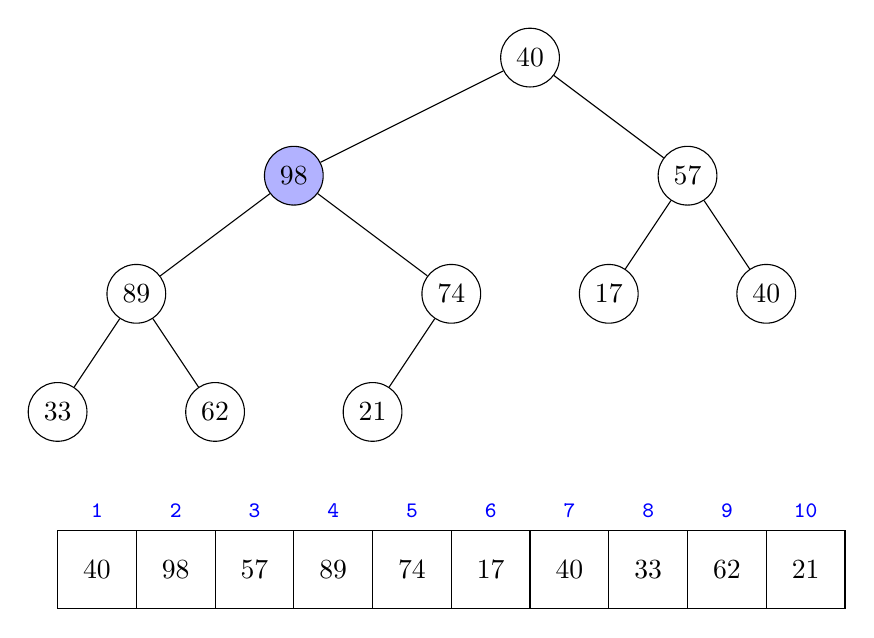
\begin{tikzpicture}
                % Sequência de inserção: 40, 98, 17, 33, 21, 57, 40, 89, 62, 74
                \node[circle,draw] (A) at (6, 6) { 40 };
                \node[circle,draw,fill=blue!30] (B) at (3, 4.5) { 98 };
                \node[circle,draw] (C) at (8, 4.5) { 57 };
                \node[circle,draw] (D) at (1, 3) { 89 };
                \node[circle,draw] (E) at (5, 3) { 74 };
                \node[circle,draw] (F) at (7, 3) { 17 };
                \node[circle,draw] (G) at (9, 3) { 40 };
                \node[circle,draw] (H) at (0, 1.5) { 33 };
                \node[circle,draw] (I) at (2, 1.5) { 62 };
                \node[circle,draw] (J) at (4, 1.5) { 21 };

                \draw (A) -- (B);
                \draw (A) -- (C);
                \draw (B) -- (D);
                \draw (B) -- (E);
                \draw (C) -- (F);
                \draw (C) -- (G);
                \draw (D) -- (H);
                \draw (D) -- (I);
                \draw (E) -- (J);

                \draw (0, -1) grid (10, 0);

                \node[color=blue] at (0.5, 0.25) { \footnotesize \texttt{\textbf{1}} };
                \node[color=blue] at (1.5, 0.25) { \footnotesize \texttt{\textbf{2}} };
                \node[color=blue] at (2.5, 0.25) { \footnotesize \texttt{\textbf{3}} };
                \node[color=blue] at (3.5, 0.25) { \footnotesize \texttt{\textbf{4}} };
                \node[color=blue] at (4.5, 0.25) { \footnotesize \texttt{\textbf{5}} };
                \node[color=blue] at (5.5, 0.25) { \footnotesize \texttt{\textbf{6}} };
                \node[color=blue] at (6.5, 0.25) { \footnotesize \texttt{\textbf{7}} };
                \node[color=blue] at (7.5, 0.25) { \footnotesize \texttt{\textbf{8}} };
                \node[color=blue] at (8.5, 0.25) { \footnotesize \texttt{\textbf{9}} };
                \node[color=blue] at (9.5, 0.25) { \footnotesize \texttt{\textbf{10}} };

                \node at (0.5, -0.5) { 40 };
                \node at (1.5, -0.5) { 98 };
                \node at (2.5, -0.5) { \textcolor{black}{57} };
                \node at (3.5, -0.5) { \textcolor{black}{89} };
                \node at (4.5, -0.5) { \textcolor{black}{74} };
                \node at (5.5, -0.5) { \textcolor{black}{17} };
                \node at (6.5, -0.5) { 40 };
                \node at (7.5, -0.5) { \textcolor{black}{33}};
                \node at (8.5, -0.5) { 62 };
                \node at (9.5, -0.5) { \textcolor{black}{21} };
        \end{tikzpicture}
    \end{figure}

\end{frame}

\begin{frame}[fragile]{Exemplo de execução da rotina \code{c}{heapify()}}

    \begin{figure}
        \centering
        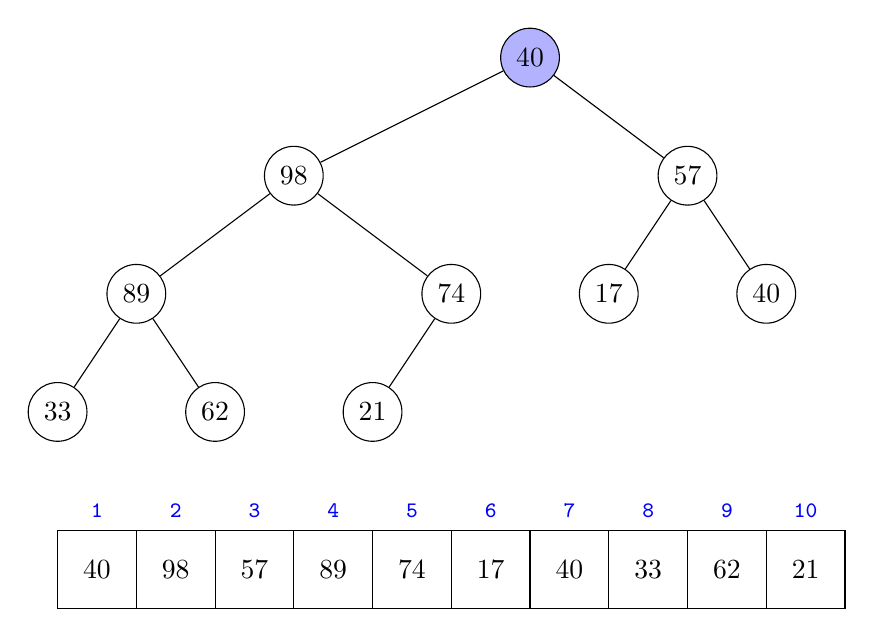
\begin{tikzpicture}
                % Sequência de inserção: 40, 98, 17, 33, 21, 57, 40, 89, 62, 74
                \node[circle,draw,fill=blue!30] (A) at (6, 6) { 40 };
                \node[circle,draw] (B) at (3, 4.5) { 98 };
                \node[circle,draw] (C) at (8, 4.5) { 57 };
                \node[circle,draw] (D) at (1, 3) { 89 };
                \node[circle,draw] (E) at (5, 3) { 74 };
                \node[circle,draw] (F) at (7, 3) { 17 };
                \node[circle,draw] (G) at (9, 3) { 40 };
                \node[circle,draw] (H) at (0, 1.5) { 33 };
                \node[circle,draw] (I) at (2, 1.5) { 62 };
                \node[circle,draw] (J) at (4, 1.5) { 21 };

                \draw (A) -- (B);
                \draw (A) -- (C);
                \draw (B) -- (D);
                \draw (B) -- (E);
                \draw (C) -- (F);
                \draw (C) -- (G);
                \draw (D) -- (H);
                \draw (D) -- (I);
                \draw (E) -- (J);

                \draw (0, -1) grid (10, 0);

                \node[color=blue] at (0.5, 0.25) { \footnotesize \texttt{\textbf{1}} };
                \node[color=blue] at (1.5, 0.25) { \footnotesize \texttt{\textbf{2}} };
                \node[color=blue] at (2.5, 0.25) { \footnotesize \texttt{\textbf{3}} };
                \node[color=blue] at (3.5, 0.25) { \footnotesize \texttt{\textbf{4}} };
                \node[color=blue] at (4.5, 0.25) { \footnotesize \texttt{\textbf{5}} };
                \node[color=blue] at (5.5, 0.25) { \footnotesize \texttt{\textbf{6}} };
                \node[color=blue] at (6.5, 0.25) { \footnotesize \texttt{\textbf{7}} };
                \node[color=blue] at (7.5, 0.25) { \footnotesize \texttt{\textbf{8}} };
                \node[color=blue] at (8.5, 0.25) { \footnotesize \texttt{\textbf{9}} };
                \node[color=blue] at (9.5, 0.25) { \footnotesize \texttt{\textbf{10}} };

                \node at (0.5, -0.5) { 40 };
                \node at (1.5, -0.5) { 98 };
                \node at (2.5, -0.5) { \textcolor{black}{57} };
                \node at (3.5, -0.5) { \textcolor{black}{89} };
                \node at (4.5, -0.5) { \textcolor{black}{74} };
                \node at (5.5, -0.5) { \textcolor{black}{17} };
                \node at (6.5, -0.5) { 40 };
                \node at (7.5, -0.5) { \textcolor{black}{33}};
                \node at (8.5, -0.5) { 62 };
                \node at (9.5, -0.5) { \textcolor{black}{21} };
        \end{tikzpicture}
    \end{figure}

\end{frame}

\begin{frame}[fragile]{Exemplo de execução da rotina \code{c}{heapify()}}

    \begin{figure}
        \centering
        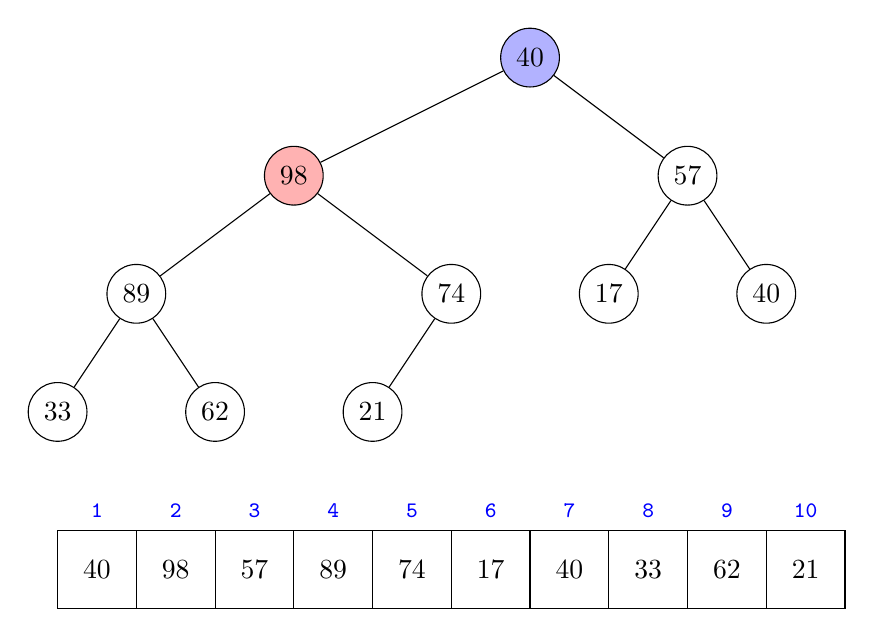
\begin{tikzpicture}
                % Sequência de inserção: 40, 98, 17, 33, 21, 57, 40, 89, 62, 74
                \node[circle,draw,fill=blue!30] (A) at (6, 6) { 40 };
                \node[circle,draw,fill=red!30] (B) at (3, 4.5) { 98 };
                \node[circle,draw] (C) at (8, 4.5) { 57 };
                \node[circle,draw] (D) at (1, 3) { 89 };
                \node[circle,draw] (E) at (5, 3) { 74 };
                \node[circle,draw] (F) at (7, 3) { 17 };
                \node[circle,draw] (G) at (9, 3) { 40 };
                \node[circle,draw] (H) at (0, 1.5) { 33 };
                \node[circle,draw] (I) at (2, 1.5) { 62 };
                \node[circle,draw] (J) at (4, 1.5) { 21 };

                \draw (A) -- (B);
                \draw (A) -- (C);
                \draw (B) -- (D);
                \draw (B) -- (E);
                \draw (C) -- (F);
                \draw (C) -- (G);
                \draw (D) -- (H);
                \draw (D) -- (I);
                \draw (E) -- (J);

                \draw (0, -1) grid (10, 0);

                \node[color=blue] at (0.5, 0.25) { \footnotesize \texttt{\textbf{1}} };
                \node[color=blue] at (1.5, 0.25) { \footnotesize \texttt{\textbf{2}} };
                \node[color=blue] at (2.5, 0.25) { \footnotesize \texttt{\textbf{3}} };
                \node[color=blue] at (3.5, 0.25) { \footnotesize \texttt{\textbf{4}} };
                \node[color=blue] at (4.5, 0.25) { \footnotesize \texttt{\textbf{5}} };
                \node[color=blue] at (5.5, 0.25) { \footnotesize \texttt{\textbf{6}} };
                \node[color=blue] at (6.5, 0.25) { \footnotesize \texttt{\textbf{7}} };
                \node[color=blue] at (7.5, 0.25) { \footnotesize \texttt{\textbf{8}} };
                \node[color=blue] at (8.5, 0.25) { \footnotesize \texttt{\textbf{9}} };
                \node[color=blue] at (9.5, 0.25) { \footnotesize \texttt{\textbf{10}} };

                \node at (0.5, -0.5) { 40 };
                \node at (1.5, -0.5) { 98 };
                \node at (2.5, -0.5) { \textcolor{black}{57} };
                \node at (3.5, -0.5) { \textcolor{black}{89} };
                \node at (4.5, -0.5) { \textcolor{black}{74} };
                \node at (5.5, -0.5) { \textcolor{black}{17} };
                \node at (6.5, -0.5) { 40 };
                \node at (7.5, -0.5) { \textcolor{black}{33}};
                \node at (8.5, -0.5) { 62 };
                \node at (9.5, -0.5) { \textcolor{black}{21} };
        \end{tikzpicture}
    \end{figure}

\end{frame}

\begin{frame}[fragile]{Exemplo de execução da rotina \code{c}{heapify()}}

    \begin{figure}
        \centering
        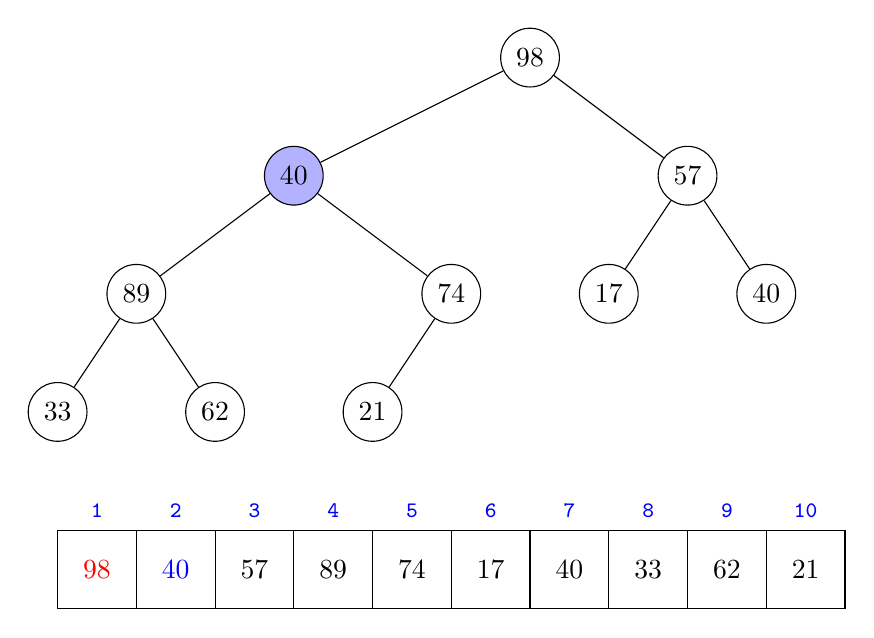
\begin{tikzpicture}
                % Sequência de inserção: 40, 98, 17, 33, 21, 57, 40, 89, 62, 74
                \node[circle,draw] (A) at (6, 6) { 98 };
                \node[circle,draw,fill=blue!30] (B) at (3, 4.5) { 40 };
                \node[circle,draw] (C) at (8, 4.5) { 57 };
                \node[circle,draw] (D) at (1, 3) { 89 };
                \node[circle,draw] (E) at (5, 3) { 74 };
                \node[circle,draw] (F) at (7, 3) { 17 };
                \node[circle,draw] (G) at (9, 3) { 40 };
                \node[circle,draw] (H) at (0, 1.5) { 33 };
                \node[circle,draw] (I) at (2, 1.5) { 62 };
                \node[circle,draw] (J) at (4, 1.5) { 21 };

                \draw (A) -- (B);
                \draw (A) -- (C);
                \draw (B) -- (D);
                \draw (B) -- (E);
                \draw (C) -- (F);
                \draw (C) -- (G);
                \draw (D) -- (H);
                \draw (D) -- (I);
                \draw (E) -- (J);

                \draw (0, -1) grid (10, 0);

                \node[color=blue] at (0.5, 0.25) { \footnotesize \texttt{\textbf{1}} };
                \node[color=blue] at (1.5, 0.25) { \footnotesize \texttt{\textbf{2}} };
                \node[color=blue] at (2.5, 0.25) { \footnotesize \texttt{\textbf{3}} };
                \node[color=blue] at (3.5, 0.25) { \footnotesize \texttt{\textbf{4}} };
                \node[color=blue] at (4.5, 0.25) { \footnotesize \texttt{\textbf{5}} };
                \node[color=blue] at (5.5, 0.25) { \footnotesize \texttt{\textbf{6}} };
                \node[color=blue] at (6.5, 0.25) { \footnotesize \texttt{\textbf{7}} };
                \node[color=blue] at (7.5, 0.25) { \footnotesize \texttt{\textbf{8}} };
                \node[color=blue] at (8.5, 0.25) { \footnotesize \texttt{\textbf{9}} };
                \node[color=blue] at (9.5, 0.25) { \footnotesize \texttt{\textbf{10}} };

                \node at (0.5, -0.5) { \textcolor{red}{98} };
                \node at (1.5, -0.5) { \textcolor{blue}{40} };
                \node at (2.5, -0.5) { \textcolor{black}{57} };
                \node at (3.5, -0.5) { \textcolor{black}{89} };
                \node at (4.5, -0.5) { \textcolor{black}{74} };
                \node at (5.5, -0.5) { \textcolor{black}{17} };
                \node at (6.5, -0.5) { 40 };
                \node at (7.5, -0.5) { \textcolor{black}{33}};
                \node at (8.5, -0.5) { 62 };
                \node at (9.5, -0.5) { \textcolor{black}{21} };
        \end{tikzpicture}
    \end{figure}

\end{frame}

\begin{frame}[fragile]{Exemplo de execução da rotina \code{c}{heapify()}}

    \begin{figure}
        \centering
        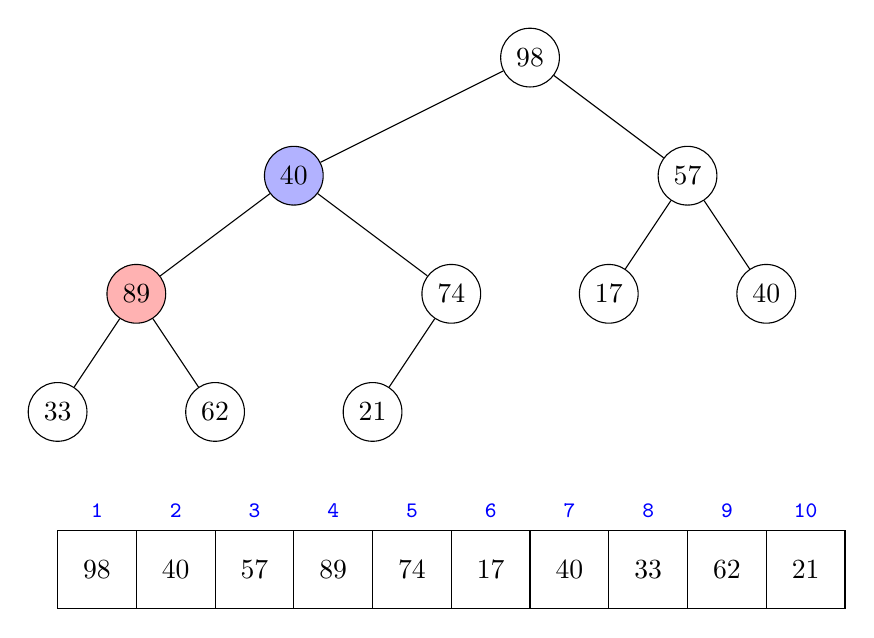
\begin{tikzpicture}
                % Sequência de inserção: 40, 98, 17, 33, 21, 57, 40, 89, 62, 74
                \node[circle,draw] (A) at (6, 6) { 98 };
                \node[circle,draw,fill=blue!30] (B) at (3, 4.5) { 40 };
                \node[circle,draw] (C) at (8, 4.5) { 57 };
                \node[circle,draw,fill=red!30] (D) at (1, 3) { 89 };
                \node[circle,draw] (E) at (5, 3) { 74 };
                \node[circle,draw] (F) at (7, 3) { 17 };
                \node[circle,draw] (G) at (9, 3) { 40 };
                \node[circle,draw] (H) at (0, 1.5) { 33 };
                \node[circle,draw] (I) at (2, 1.5) { 62 };
                \node[circle,draw] (J) at (4, 1.5) { 21 };

                \draw (A) -- (B);
                \draw (A) -- (C);
                \draw (B) -- (D);
                \draw (B) -- (E);
                \draw (C) -- (F);
                \draw (C) -- (G);
                \draw (D) -- (H);
                \draw (D) -- (I);
                \draw (E) -- (J);

                \draw (0, -1) grid (10, 0);

                \node[color=blue] at (0.5, 0.25) { \footnotesize \texttt{\textbf{1}} };
                \node[color=blue] at (1.5, 0.25) { \footnotesize \texttt{\textbf{2}} };
                \node[color=blue] at (2.5, 0.25) { \footnotesize \texttt{\textbf{3}} };
                \node[color=blue] at (3.5, 0.25) { \footnotesize \texttt{\textbf{4}} };
                \node[color=blue] at (4.5, 0.25) { \footnotesize \texttt{\textbf{5}} };
                \node[color=blue] at (5.5, 0.25) { \footnotesize \texttt{\textbf{6}} };
                \node[color=blue] at (6.5, 0.25) { \footnotesize \texttt{\textbf{7}} };
                \node[color=blue] at (7.5, 0.25) { \footnotesize \texttt{\textbf{8}} };
                \node[color=blue] at (8.5, 0.25) { \footnotesize \texttt{\textbf{9}} };
                \node[color=blue] at (9.5, 0.25) { \footnotesize \texttt{\textbf{10}} };

                \node at (0.5, -0.5) { \textcolor{black}{98} };
                \node at (1.5, -0.5) { \textcolor{black}{40} };
                \node at (2.5, -0.5) { \textcolor{black}{57} };
                \node at (3.5, -0.5) { \textcolor{black}{89} };
                \node at (4.5, -0.5) { \textcolor{black}{74} };
                \node at (5.5, -0.5) { \textcolor{black}{17} };
                \node at (6.5, -0.5) { 40 };
                \node at (7.5, -0.5) { \textcolor{black}{33}};
                \node at (8.5, -0.5) { 62 };
                \node at (9.5, -0.5) { \textcolor{black}{21} };
        \end{tikzpicture}
    \end{figure}

\end{frame}

\begin{frame}[fragile]{Exemplo de execução da rotina \code{c}{heapify()}}

    \begin{figure}
        \centering
        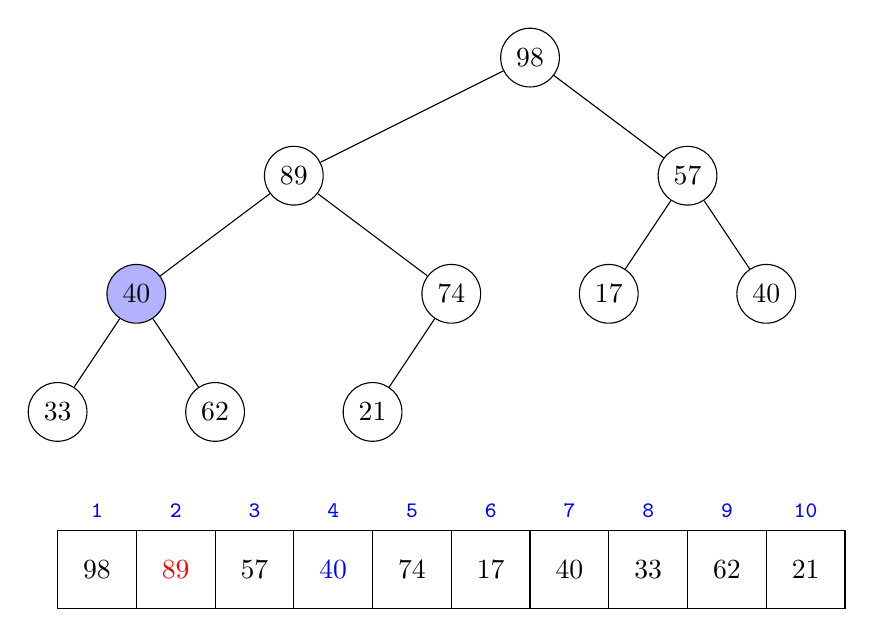
\begin{tikzpicture}
                % Sequência de inserção: 40, 98, 17, 33, 21, 57, 40, 89, 62, 74
                \node[circle,draw] (A) at (6, 6) { 98 };
                \node[circle,draw] (B) at (3, 4.5) { 89 };
                \node[circle,draw] (C) at (8, 4.5) { 57 };
                \node[circle,draw,fill=blue!30] (D) at (1, 3) { 40 };
                \node[circle,draw] (E) at (5, 3) { 74 };
                \node[circle,draw] (F) at (7, 3) { 17 };
                \node[circle,draw] (G) at (9, 3) { 40 };
                \node[circle,draw] (H) at (0, 1.5) { 33 };
                \node[circle,draw] (I) at (2, 1.5) { 62 };
                \node[circle,draw] (J) at (4, 1.5) { 21 };

                \draw (A) -- (B);
                \draw (A) -- (C);
                \draw (B) -- (D);
                \draw (B) -- (E);
                \draw (C) -- (F);
                \draw (C) -- (G);
                \draw (D) -- (H);
                \draw (D) -- (I);
                \draw (E) -- (J);

                \draw (0, -1) grid (10, 0);

                \node[color=blue] at (0.5, 0.25) { \footnotesize \texttt{\textbf{1}} };
                \node[color=blue] at (1.5, 0.25) { \footnotesize \texttt{\textbf{2}} };
                \node[color=blue] at (2.5, 0.25) { \footnotesize \texttt{\textbf{3}} };
                \node[color=blue] at (3.5, 0.25) { \footnotesize \texttt{\textbf{4}} };
                \node[color=blue] at (4.5, 0.25) { \footnotesize \texttt{\textbf{5}} };
                \node[color=blue] at (5.5, 0.25) { \footnotesize \texttt{\textbf{6}} };
                \node[color=blue] at (6.5, 0.25) { \footnotesize \texttt{\textbf{7}} };
                \node[color=blue] at (7.5, 0.25) { \footnotesize \texttt{\textbf{8}} };
                \node[color=blue] at (8.5, 0.25) { \footnotesize \texttt{\textbf{9}} };
                \node[color=blue] at (9.5, 0.25) { \footnotesize \texttt{\textbf{10}} };

                \node at (0.5, -0.5) { \textcolor{black}{98} };
                \node at (1.5, -0.5) { \textcolor{red}{89} };
                \node at (2.5, -0.5) { \textcolor{black}{57} };
                \node at (3.5, -0.5) { \textcolor{blue}{40} };
                \node at (4.5, -0.5) { \textcolor{black}{74} };
                \node at (5.5, -0.5) { \textcolor{black}{17} };
                \node at (6.5, -0.5) { 40 };
                \node at (7.5, -0.5) { \textcolor{black}{33}};
                \node at (8.5, -0.5) { 62 };
                \node at (9.5, -0.5) { \textcolor{black}{21} };
        \end{tikzpicture}
    \end{figure}

\end{frame}

\begin{frame}[fragile]{Exemplo de execução da rotina \code{c}{heapify()}}

    \begin{figure}
        \centering
        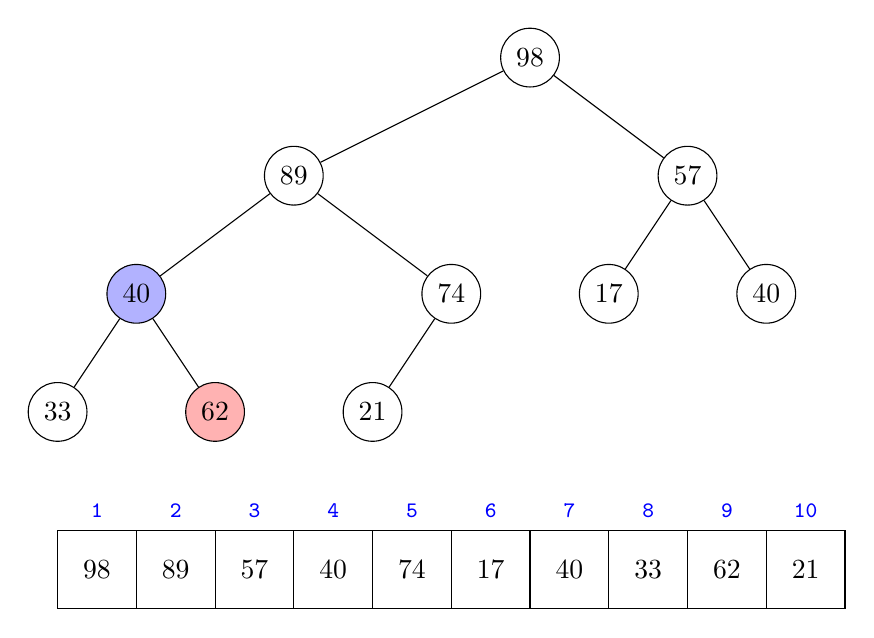
\begin{tikzpicture}
                % Sequência de inserção: 40, 98, 17, 33, 21, 57, 40, 89, 62, 74
                \node[circle,draw] (A) at (6, 6) { 98 };
                \node[circle,draw] (B) at (3, 4.5) { 89 };
                \node[circle,draw] (C) at (8, 4.5) { 57 };
                \node[circle,draw,fill=blue!30] (D) at (1, 3) { 40 };
                \node[circle,draw] (E) at (5, 3) { 74 };
                \node[circle,draw] (F) at (7, 3) { 17 };
                \node[circle,draw] (G) at (9, 3) { 40 };
                \node[circle,draw] (H) at (0, 1.5) { 33 };
                \node[circle,draw,fill=red!30] (I) at (2, 1.5) { 62 };
                \node[circle,draw] (J) at (4, 1.5) { 21 };

                \draw (A) -- (B);
                \draw (A) -- (C);
                \draw (B) -- (D);
                \draw (B) -- (E);
                \draw (C) -- (F);
                \draw (C) -- (G);
                \draw (D) -- (H);
                \draw (D) -- (I);
                \draw (E) -- (J);

                \draw (0, -1) grid (10, 0);

                \node[color=blue] at (0.5, 0.25) { \footnotesize \texttt{\textbf{1}} };
                \node[color=blue] at (1.5, 0.25) { \footnotesize \texttt{\textbf{2}} };
                \node[color=blue] at (2.5, 0.25) { \footnotesize \texttt{\textbf{3}} };
                \node[color=blue] at (3.5, 0.25) { \footnotesize \texttt{\textbf{4}} };
                \node[color=blue] at (4.5, 0.25) { \footnotesize \texttt{\textbf{5}} };
                \node[color=blue] at (5.5, 0.25) { \footnotesize \texttt{\textbf{6}} };
                \node[color=blue] at (6.5, 0.25) { \footnotesize \texttt{\textbf{7}} };
                \node[color=blue] at (7.5, 0.25) { \footnotesize \texttt{\textbf{8}} };
                \node[color=blue] at (8.5, 0.25) { \footnotesize \texttt{\textbf{9}} };
                \node[color=blue] at (9.5, 0.25) { \footnotesize \texttt{\textbf{10}} };

                \node at (0.5, -0.5) { \textcolor{black}{98} };
                \node at (1.5, -0.5) { \textcolor{black}{89} };
                \node at (2.5, -0.5) { \textcolor{black}{57} };
                \node at (3.5, -0.5) { \textcolor{black}{40} };
                \node at (4.5, -0.5) { \textcolor{black}{74} };
                \node at (5.5, -0.5) { \textcolor{black}{17} };
                \node at (6.5, -0.5) { 40 };
                \node at (7.5, -0.5) { \textcolor{black}{33}};
                \node at (8.5, -0.5) { 62 };
                \node at (9.5, -0.5) { \textcolor{black}{21} };
        \end{tikzpicture}
    \end{figure}

\end{frame}

\begin{frame}[fragile]{Exemplo de execução da rotina \code{c}{heapify()}}

    \begin{figure}
        \centering
        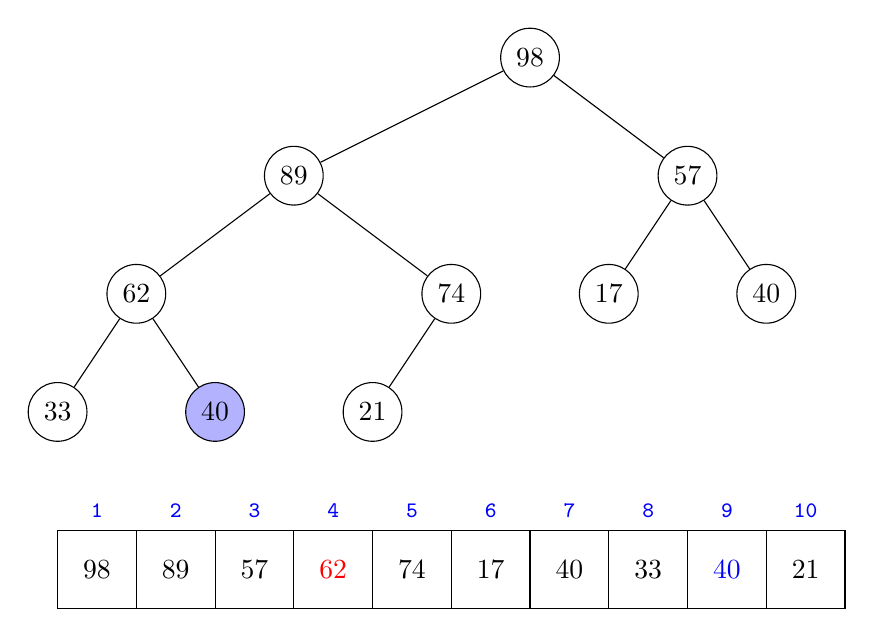
\begin{tikzpicture}
                % Sequência de inserção: 40, 98, 17, 33, 21, 57, 40, 89, 62, 74
                \node[circle,draw] (A) at (6, 6) { 98 };
                \node[circle,draw] (B) at (3, 4.5) { 89 };
                \node[circle,draw] (C) at (8, 4.5) { 57 };
                \node[circle,draw] (D) at (1, 3) { 62 };
                \node[circle,draw] (E) at (5, 3) { 74 };
                \node[circle,draw] (F) at (7, 3) { 17 };
                \node[circle,draw] (G) at (9, 3) { 40 };
                \node[circle,draw] (H) at (0, 1.5) { 33 };
                \node[circle,draw,fill=blue!30] (I) at (2, 1.5) { 40 };
                \node[circle,draw] (J) at (4, 1.5) { 21 };

                \draw (A) -- (B);
                \draw (A) -- (C);
                \draw (B) -- (D);
                \draw (B) -- (E);
                \draw (C) -- (F);
                \draw (C) -- (G);
                \draw (D) -- (H);
                \draw (D) -- (I);
                \draw (E) -- (J);

                \draw (0, -1) grid (10, 0);

                \node[color=blue] at (0.5, 0.25) { \footnotesize \texttt{\textbf{1}} };
                \node[color=blue] at (1.5, 0.25) { \footnotesize \texttt{\textbf{2}} };
                \node[color=blue] at (2.5, 0.25) { \footnotesize \texttt{\textbf{3}} };
                \node[color=blue] at (3.5, 0.25) { \footnotesize \texttt{\textbf{4}} };
                \node[color=blue] at (4.5, 0.25) { \footnotesize \texttt{\textbf{5}} };
                \node[color=blue] at (5.5, 0.25) { \footnotesize \texttt{\textbf{6}} };
                \node[color=blue] at (6.5, 0.25) { \footnotesize \texttt{\textbf{7}} };
                \node[color=blue] at (7.5, 0.25) { \footnotesize \texttt{\textbf{8}} };
                \node[color=blue] at (8.5, 0.25) { \footnotesize \texttt{\textbf{9}} };
                \node[color=blue] at (9.5, 0.25) { \footnotesize \texttt{\textbf{10}} };

                \node at (0.5, -0.5) { \textcolor{black}{98} };
                \node at (1.5, -0.5) { \textcolor{black}{89} };
                \node at (2.5, -0.5) { \textcolor{black}{57} };
                \node at (3.5, -0.5) { \textcolor{red}{62} };
                \node at (4.5, -0.5) { \textcolor{black}{74} };
                \node at (5.5, -0.5) { \textcolor{black}{17} };
                \node at (6.5, -0.5) { 40 };
                \node at (7.5, -0.5) { \textcolor{black}{33}};
                \node at (8.5, -0.5) { \textcolor{blue}{40} };
                \node at (9.5, -0.5) { \textcolor{black}{21} };
        \end{tikzpicture}
    \end{figure}

\end{frame}

\begin{frame}[fragile]{Exemplo de execução da rotina \code{c}{heapify()}}

    \begin{figure}
        \centering
        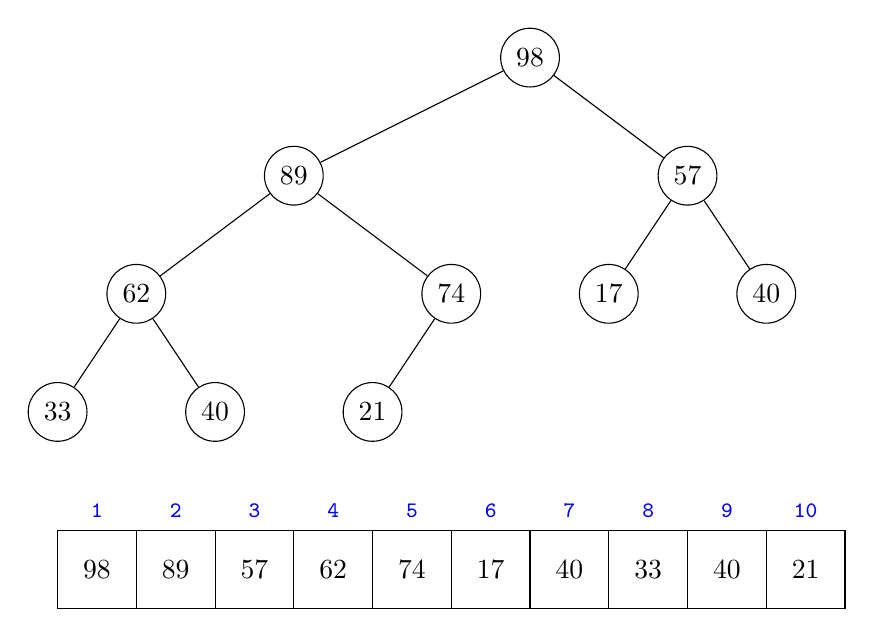
\begin{tikzpicture}
                % Sequência de inserção: 40, 98, 17, 33, 21, 57, 40, 89, 62, 74
                \node[circle,draw] (A) at (6, 6) { 98 };
                \node[circle,draw] (B) at (3, 4.5) { 89 };
                \node[circle,draw] (C) at (8, 4.5) { 57 };
                \node[circle,draw] (D) at (1, 3) { 62 };
                \node[circle,draw] (E) at (5, 3) { 74 };
                \node[circle,draw] (F) at (7, 3) { 17 };
                \node[circle,draw] (G) at (9, 3) { 40 };
                \node[circle,draw] (H) at (0, 1.5) { 33 };
                \node[circle,draw] (I) at (2, 1.5) { 40 };
                \node[circle,draw] (J) at (4, 1.5) { 21 };

                \draw (A) -- (B);
                \draw (A) -- (C);
                \draw (B) -- (D);
                \draw (B) -- (E);
                \draw (C) -- (F);
                \draw (C) -- (G);
                \draw (D) -- (H);
                \draw (D) -- (I);
                \draw (E) -- (J);

                \draw (0, -1) grid (10, 0);

                \node[color=blue] at (0.5, 0.25) { \footnotesize \texttt{\textbf{1}} };
                \node[color=blue] at (1.5, 0.25) { \footnotesize \texttt{\textbf{2}} };
                \node[color=blue] at (2.5, 0.25) { \footnotesize \texttt{\textbf{3}} };
                \node[color=blue] at (3.5, 0.25) { \footnotesize \texttt{\textbf{4}} };
                \node[color=blue] at (4.5, 0.25) { \footnotesize \texttt{\textbf{5}} };
                \node[color=blue] at (5.5, 0.25) { \footnotesize \texttt{\textbf{6}} };
                \node[color=blue] at (6.5, 0.25) { \footnotesize \texttt{\textbf{7}} };
                \node[color=blue] at (7.5, 0.25) { \footnotesize \texttt{\textbf{8}} };
                \node[color=blue] at (8.5, 0.25) { \footnotesize \texttt{\textbf{9}} };
                \node[color=blue] at (9.5, 0.25) { \footnotesize \texttt{\textbf{10}} };

                \node at (0.5, -0.5) { \textcolor{black}{98} };
                \node at (1.5, -0.5) { \textcolor{black}{89} };
                \node at (2.5, -0.5) { \textcolor{black}{57} };
                \node at (3.5, -0.5) { \textcolor{black}{62} };
                \node at (4.5, -0.5) { \textcolor{black}{74} };
                \node at (5.5, -0.5) { \textcolor{black}{17} };
                \node at (6.5, -0.5) { 40 };
                \node at (7.5, -0.5) { \textcolor{black}{33}};
                \node at (8.5, -0.5) { \textcolor{black}{40} };
                \node at (9.5, -0.5) { \textcolor{black}{21} };
        \end{tikzpicture}
    \end{figure}

\end{frame}

\begin{frame}[fragile]{Implementação da rotina \code{c}{heapify()}}
    \inputsnippet{cpp}{79}{98}{codes/heap.cpp}
\end{frame}

\begin{frame}[fragile]{Implementação da rotina \code{c}{heapify()}}
    \inputsnippet{cpp}{100}{112}{codes/heap.cpp}
\end{frame}

\begin{frame}[fragile]{Complexidade da rotina \code{c}{heapify()}}

    \begin{itemize}
        \item Seja $h = \lfloor \log N\rfloor$ a altura da \textit{heap} binária

        \item O número de nós $V$ no nível $i$ é tal que
        \[
            V(i) \leq 2^i \leq \frac{2^{\lfloor \log N\rfloor}}{2^{h - i}} \leq \frac{n}{2^{h - i}}
        \]

        \item O número de trocas máximas para um nó no nível $i$ é $O(h - i)$

        \item Assim, o total $T$ de trocas feitas será dado por
        \begin{align*}
            T &= \sum_{i = 0}^h V(i)O(h - i) = \sum_{i = 0}^{\lfloor \log N\rfloor} \frac{n}{2^{h - i}}O(h - i) =
                \sum_{k = 0}^{\lfloor \log N\rfloor} \frac{n}{2^{k}}O(k) \\
              &=  O\left(n\sum_{k = 0}^{\lfloor \log N\rfloor} \frac{k}{2^{k}}\right)
              \leq  O\left(n\sum_{k = 0}^{\infty} \frac{k}{2^{k}}\right) = O(n),
        \end{align*}
        pois a série infinita $a_k = \sum k/2^k$ converge

    \end{itemize}

\end{frame}
